\documentclass[final,3p,times,11pt]{elsarticle}
\usepackage[USenglish]{babel}
\usepackage{amsmath,amssymb,amsthm, mathrsfs,multirow}
\usepackage{mathtools}
\usepackage{graphicx}
\usepackage{stmaryrd}
\usepackage[dvipsnames]{xcolor}
\usepackage{cancel}
\usepackage{ulem}
\usepackage{tabularx}
\usepackage{comment}
%\usepackage{subcaption}
%\usepackage[show]{ed}
%\usepackage{showkeys}
%\usepackage{showlabels}
%\usepackage[notcite,notref]{showkeys}
%\usepackage{refcheck}
% \usepackage[ruled,vlined]{algorithm2e}
\usepackage[linesnumbered,ruled,vlined]{algorithm2e}
\definecolor{Myblue}{rgb}{.2 0.4 1}

\usepackage{hyperref}
\hypersetup{
    %bookmarks=true,         % show bookmarks bar?
    colorlinks = true,       % false: boxed links; true: colored links
    % linkcolor=green
     %linkcolor=red,          % color of internal links (change box color with linkbordercolor)
     %citecolor=green,        % color of links to bibliography
    %filecolor=magenta,      % color of file links
    %urlcolor=cyan           % color of external links
}
%\usepackage{wrapfig}
%% The lineno packages adds line numbers. Start line numbering with
%% \begin{linenumbers}, end it with \end{linenumbers}. Or switch it on
%% for the whole article with \linenumbers after \end{frontmatter}.
%\usepackage{lineno}


% ==============   Macros  ====================
\newcommand{\mynabla}{\widetilde{\nabla}} 
\newcommand{\jump}[1]{[\![#1]\!]}
\newcommand{\HEcolor}[1]{{\textcolor{blue}{#1}}}
\newcommand{\TSVcolor}[1]{{\textcolor{orange}{#1}}}
\newcommand{\JLcolor}[1]{{\textcolor{violet}{#1}}} %violet
\newcommand{\Grids}{\boldsymbol{\chi}}

\newtheorem{theorem}{Theorem}%[section]
\newtheorem{VariationalForm}[theorem]{Variational Formulation}
% =============================================

\journal{}
\makeatletter
\def\ps@pprintTitle{%
 \let\@oddhead\@empty
 \let\@evenhead\@empty
 \def\@oddfoot{}%
 \let\@evenfoot\@oddfoot}
\makeatother




\begin{document}
\begin{frontmatter}
\title{Multi-fidelity Monte Carlo for uncertainty quantification in the free boundary Grad-Shafranov equation}


\author[umdcs]{Matthias Heinkenschloss}
\ead{heinken@rice.edu}
\address[umdcs]{Department of Computational Applied Mathematics \& Operations Research, Rice University.}
\author[umdm]{Jiaxing Liang}
\ead{jl508@rice.edu}
\address[umdm]{Department of Computational Applied Mathematics \& Operations Research, Rice University.}
% \author[UA]{Tonatiuh S\'anchez-Vizuet}
% \ead{tonatiuh@arizona.edu}
% \address[UA]{Department of Mathematics, The University of Arizona.}
\begin{abstract}
We investigate the Grad-Shafranov free boundary problem in Tokamak fusion reactors under the influence of parameter uncertainties. Using both traditional Monte Carlo and multi-fidelity Monte Carlo sampling approaches, we quantify the impact of these uncertainties on model predictions, emphasizing the statistical characterization of solution variability across diverse parameter regimes. Our numerical results reveals that the multi-fidelity Monte Carlo estimator achieves statistical accuracy comparable to the Monte Carlo approach. However, the multi-fidelity method demonstrates superior computational efficiency, achieving a cost reduction by a factor of ..., while preserving fidelity in representing plasma boundary dynamics and geometric parameters. This work underscores the efficiency of multi-fidelity frameworks in addressing the computational demands of uncertainty quantification in complex fusion reactor models, offering a robust pathway for enhancing predictive capabilities in plasma physics. 
\end{abstract}

\begin{keyword}
Multi-fidelity Monte Carlo Finite-Element \sep Parametric expectation, \sep Sparse Grid Stochastic Collocation \sep Uncertainty Quantification \sep Free Boundary Grad-Shafranov Problem.
%
\MSC[2020] 
\end{keyword}
\end{frontmatter}

%!TEX root = main.tex
%%%%%%%%%%%%%%%%%%%%%%%%%%%%%%%%%%%%%%%%%%%%%%%%%%%

% ========================================
\section{Introduction}\label{sec:intro}
% ========================================
The Monte Carlo (MC) method is a fundamental tool for uncertainty quantification in computational science and engineering. It estimates statistical properties of quantities influenced by stochastic inputs through repeated evaluations of a deterministic model. Its non-intrusive nature and broad applicability -- requiring no assumptions about the smoothness or structure of the input distributions -- make it widely appealing. However, a key limitation of the MC method is its slow convergence rate of $1/\sqrt{N}$, where $N$ is the number of samples, which leads to high computational costs, particularly when the evaluation of each model is expensive. Such costs are especially pronounced in the context of non-linear partial differential equations (PDEs), which typically require high-fidelity numerical discretizations -- such as fine-mesh finite element methods -- to accurately resolve the solution. Consequently, direct application of standard MC methods to these problems can become computationally prohibitive. To mitigate this burden, surrogate models have been developed as low-fidelity approximations that retain essential features of the high-fidelity model while offering substantial reductions in cost. These models accelerate sampling by approximating the underlying system at coarser resolution or through simplified representations while retaining sufficient accuracy for statistical inference. However, the simplifications inherent in surrogate construction can introduce bias and reduce accuracy, particularly in regions where the surrogate fails to capture important solution features. For instance, \cite{ElLiSa:2022} demonstrates that surrogate models based on stochastic collocation can significantly accelerate MC sampling while maintaining reliable accuracy. An alternative strategy to accelerate Monte Carlo sampling is provided by the multilevel Monte Carlo (MLMC) method \cite{BaScZo:2011,Gi:2008,Gi:2015}, which constructs a hierarchy of spatial discretizations to efficiently estimate statistical quantities. The key idea is to compute most of the variance contribution using inexpensive coarse-grid models, while reserving costly fine-grid evaluations for corrections at the highest resolution. This hierarchical approach significantly reduces the total computational cost compared to standard MC methods. For example, \cite{ElLiSa:2023} investigates the application of MLMC for uncertainty quantification in PDEs, demonstrating its effectiveness in reducing computational burden. In this paper, we address these limitations by adopting the multifidelity Monte Carlo (MFMC) framework \cite{PeGuWi:2018,PeWiGu:2016,PeGuWi:2018}, which generalizes the multilevel paradigm by combining models of varying fidelity through control variates. Unlike MLMC, MFMC does not require a nested hierarchy of discretizations, allowing for greater flexibility in the selection and integration of surrogate models. While MFMC incurs some upfront cost associated with surrogate construction and variance estimation, it offers some computational savings over both standard MC and MLMC, especially in regimes where low-fidelity models are inexpensive yet sufficiently accurate to inform high-fidelity predictions.



The paper is organized as follows. Section~\ref{sec:Grad-Shafranov} introduces the Grad-Shafranov free boundary problem under uncertainty. Section~\ref{sec:SC} reviews the sparse grid stochastic collocation technique, which serves as the foundation for constructing low-fidelity models in the MFMC framework. Sections~\ref{sec:MC} and~\ref{sec:MFMC} present the Monte Carlo finite element method and its multifidelity extension, respectively. As the discussion of MLMC closely follows \cite{ElLiSa:2025}, we do not provide a detailed exposition in this work. Finally, Section~\ref{sec:Num-Exp} reports numerical experiments evaluating the efficiency and accuracy of the proposed methods.

 
 Other literature
\cite{NAretz_MGunzburger_MMorlighem_KWillcox_2025a}
\cite{AAGorodetsky_GGeraci_MSEldred_JDJakeman_2020a}



% Finally, the paper concludes with Section \ref{sec:Conclusion}, summarizing the key findings and contributions. 
% An appendix is included, containing technical mathematical details and proofs relevant to the problem and methods discussed.


 
% ========================================
\section{The Grad-Shafranov free boundary problem with uncertainty}\label{sec:Grad-Shafranov}
% ========================================
The pursuit of controlled nuclear fusion as a clean, abundant energy source has spurred intensive research into magnetic confinement. We consider fusion in an ITER-class tokamak -- a toroidal device that confines high-temperature plasma using magnetic fields. A deuterium–tritium gas mixture is injected into the chamber and heated above 100 million degrees Celsius, forming a fully ionized plasma in which fusion occurs as thermal energy overcomes Coulomb repulsion. To prevent energy loss and damage, contact between plasma and vessel walls must be avoided. Since the plasma consists of charged particles, its motion can be controlled by magnetic fields. Confinement is achieved by balancing the plasma’s internal pressure against magnetic pressure from external coils and self-induced plasma currents. The resulting equilibrium, governed by Maxwell’s equations and force balance, is described by the Grad–Shafranov equation \cite{GrRu:1958, LuSc:1957, Shafranov:1958}. Assuming axisymmetry (i.e., no dependence on the toroidal angle $\varphi$), the three-dimensional problem reduces to a two-dimensional problem in the $(r, z)$ plane, where the poloidal flux function $u(r,z)$ satisfies
%
\begin{subequations}\label{eq:FreeBoundary}
\begin{equation}\label{eq:FreeBoundary_GS}
 -\nabla\,\cdot\,\left(\frac{1}{\mu r}\nabla u\right) = \left\{ \begin{array}{ll}
r\frac{d}{d u} p(u) + \frac{1}{2\,\mu r} \frac{d}{d u} g^2(u) & \text{ in } \Omega_p(u) \\
I_k/S_k & \text{ in } \Omega_{C_k} \\
0 & \text{ elsewhere, } 
\end{array}\right.
\end{equation}
%
where $\nabla$ and $\nabla \cdot$ denote gradient and divergence operator in Cartesian coordinates; the magnetic permeability $\mu$ is constant (equal to $\mu_0$) in vacuum regions and may vary within ferromagnetic materials as a function $\mu = \mu(|\nabla u|^2/r^2)$; the domain $\Omega_p$ represents the plasma region, while $\Omega_{C_k}$ corresponds to the region occupied by the $k$-th poloidal field coil $k$ carrying current $I_k$ distributed over a cross-sectional area $S_k$. The source term in $\Omega_p$ models the toroidal plasma current density, which depends nonlinearly on $u$ in terms of the hydrostatic pressure $p(u)$ and toroidal magnetic field $g(u)$. Following the formulation in \cite{LuBr:1982}, we define 
%
\begin{equation}\label{eq:source}
\frac{d}{d u}p( u) = j_0\frac{\beta}{r_0}\left(1-u_N^{\alpha_1}\right)^{\alpha_2},  \qquad \qquad
\frac{1}{2}\frac{d}{d u}g^2(u) = j_0\mu_0r_0(1-\beta)\left(1-u_N^{\alpha_1}\right)^{\alpha_2},
\end{equation}
\end{subequations}
%
where $u_N \in [0,1]$ is the normalized poloidal flux, scaled between its values on the \textit{magnetic axis} and the plasma boundary; the parameters $r_0$, $\alpha_1$, and $\alpha_2$ characterize the outer radius of the vacuum chamber and control the sharpness of the current profile, while $\beta$ (the poloidal beta) measures the ratio of plasma pressure to magnetic pressure. The plasma boundary $\partial \Omega_p$, which depends on the solution $u$ and is defined by the last closed streamline, introduces a free-boundary aspect to the problem. The problem is further complicated by nonlinear dependencies in the boundary location, source terms, and possibly spatially varying permeability.



Let $\Omega$ be a bounded Lipschitz domain enclosing the confinement region $\Omega_p$, the external coils $\Omega_{c_i}$, and surrounding structural components.  Following \cite{Gr:1999}, the solution space $Z$ for \eqref{eq:FreeBoundary} is defined as
%
\begin{equation}\label{eq:Soln_space}
    Z:=\left\{u:\Omega\rightarrow \mathbb{R} \,\Bigg| \,\int_\Omega u^2rdrdz<\infty; \,  \int_\Omega\frac{|\nabla u|^2}{r}drdz<\infty; \, u(0,z)=0 \right\}\cap C^0(\overline{\Omega}),
\end{equation}
%
equipped with the inner product and norm
%
\[
    \langle u,v\rangle_Z := \int_{\Omega} \frac{1}{r} \nabla u\cdot\nabla v \;\;drdz,\qquad \| u \|_{Z} :=\left(\int_\Omega\frac{|\nabla u|^2}{r} drdz\right)^{1/2}.
\]
%

In practice, The equilibrium configuration is sensitive to uncertainties from measurement error, modeling assumptions, and operational variability, which propagate through the system and impact both the solution $u$ and derived quantities such as the plasma boundary and $x$-point locations. In this work, we focus on uncertainties in the coil current intensities. We model the uncertainty using a $d$-dimensional random vector $\boldsymbol{\omega} = (\omega_1, \ldots, \omega_d)$, where each $\omega_k$ is an independent random variable uniformly distributed around the baseline value $\widetilde{\omega}_k$ for some relative perturbation magnitude $\tau > 0$. The corresponding joint density is
%
\[
\pi \left(\boldsymbol{\omega}\right)=\prod_{k=1}^{d} \frac{1}{2\tau |\widetilde{\omega}_k|},\quad W=\prod_{k=1}^{d}\left[\widetilde{\omega}_k-\tau \left\vert \widetilde{\omega}_k\right\vert,\widetilde{\omega}_k+\tau \left\vert \widetilde{\omega}_k \right\vert\right].
\]
%
Incorporating uncertainty into the coil currents requires solving a parameterized version of the free-boundary problem \eqref{eq:FreeBoundary}, with solution operator $u(\cdot,\boldsymbol{\omega}) : W \to Z$ mapping each realization of $\boldsymbol{\omega}$ to a solution in $Z$. To quantify the variability introduced by stochastic parameters, we adopt the {\it weighted Bochner space}. We consider the Bochner space $L^2(W,Z)$, which consists of strongly measurable functions with finite second moments defined as
% %
% \begin{equation}
% \label{eq:ParameterSpace}
%  \pi \left(\boldsymbol{\omega}\right)=\prod_{k=1}^{d} \pi_k\left(\omega_{k}\right)=\prod_{k=1}^{d} \frac{1}{2\tau |\widetilde{\omega}_k|}, \qquad  
%     W := \prod_{k=1}^{d}\left[\widetilde{\omega}_k-\tau \left\vert \widetilde{\omega}_k\right\vert,\widetilde{\omega}_k+\tau \left\vert \widetilde{\omega}_k \right\vert\right].
% \end{equation}
% %
%
\[
L^2(W,Z) = \left\{u:W\rightarrow Z\; \bigg\vert \;\int_{W}\left\|u(\cdot,\boldsymbol{\omega})\right\|_{Z}^2\pi(\boldsymbol{\omega})d\boldsymbol{\omega}<\infty\right\},
\]
%
with the associated norm on $L^2(W,Z)$ is given by
%
\[
\left\Vert u \right\Vert_{L^2(\boldsymbol W,Z)} =
    \left(\int_{\boldsymbol W} \left\Vert u(\cdot,\boldsymbol{\omega})  \right\Vert_{Z}^2 \pi(\boldsymbol{\omega})d\boldsymbol{\omega} \right)^{1/2} = \left(\mathbb{E}\left[\left\Vert u(\cdot,\boldsymbol{\omega})  \right\Vert_{Z}^2\right]\right)^{1/2}\,. 
\]
%

The objective of this paper is to investigate the propagation of uncertainty and to efficiently approximate the parametric expectation
%
 \begin{equation}
 \label{eq:QoI}
      \mathbb{E}\left(u(\cdot,\boldsymbol \omega)\right)=\int_W u(\cdot,\boldsymbol{\omega})\pi(\boldsymbol\omega)d\boldsymbol{\omega},
 \end{equation}
%
along with derived quantities from \eqref{eq:QoI} such as the plasma boundary and features of the solution, including the location of $x$-points.







% Incorporating the uncertainty and 
% %
% \begin{equation}\label{eq:FreeBoundarya}
%  -\nabla\,\cdot\,\left(\frac{1}{\mu(u(\cdot, \boldsymbol{\omega})) r}\nabla u(\cdot, \boldsymbol{\omega})\right) = \left\{ \begin{array}{ll}
% \frac{d}{du} p(u(\cdot, \boldsymbol{\omega})) + \frac{1}{2\,\mu r} \frac{d}{du} g^2(u(\cdot, \boldsymbol{\omega})) & \text{ in } \Omega_p(u(\cdot, \boldsymbol{\omega})) \\
% I_k(\boldsymbol\omega)/S_k & \text{ in } \Omega_{C_k} \\
% 0 & \text{ elsewhere, } 
% \end{array}\right.
% \end{equation}
 
% ============================================================
\section{Sparse grid stochastic collocation}\label{sec:SC}
% ============================================================
We briefly outline the sparse grid stochastic collocation method \cite{BaNoRi:2000, KlBa:2005, MaNi:2009, Sm:1963} using a generic solution $u$ for illustration. Starting from a univariate set of $m_i$ collocation nodes $X^i = \left\{x_1^i,\ldots, x_{m_i}^i\right\}$ over $[-1,1]$, the univariate interpolation operator is
%
\[
I_{X^{i}}[u]:=\sum_{j=1}^{m_{i}} u(\cdot, x_j^i)\phi_j,
\]
%
where $\phi_j$ are Lagrange basis functions satisfying $\phi_j(x_k^i) = \delta_{jk}$. To extend this construction to a $d$-dimensional parameter space,  tensor products of univariate operators are constructed. Rather than using a full tensor grid, which suffers from exponential growth in $d$, the sparse grid approach selects a reduced set of nodes per dimension to build a sparse approximation. At {\it level} $q\; (\text{where }q\ge d)$, the sparse grid nodes are
%
\begin{equation*}
H(q,d) = \bigcup_{q-d+1\le|\boldsymbol{i}|\le q} \left(X^{i_1}\times \cdots\times X^{i_d}\right)\in [-1,1]^d, 
\end{equation*}
%
where $|\boldsymbol{i}| = i_1+\ldots+i_d$ specifies the refinement rule. These nodes yield a sparse but sufficiently rich representation of the domain, capturing key features of $u$ with far fewer evaluations than a full grid.

We use Chebyshev extrema as collocation nodes \cite{BaNoRi:2000, ClCu:1960}, defined by $x_j^i=-\cos(\frac{ \pi(j-1)}{m_i-1})$ for $j=1, \ldots, m_i$ with $m_1 =1$ and $m_i = 2^{i-1}+1$ for $i\ge 2$, ensuring nestedness $X^i\subset X^{i+1}$. The corresponding multidimensional sparse grid nodes satisfy 
%
\begin{equation}
\label{eq:NestedColPts}
H(q,d)\subset H(q+1,d),\quad \text{and}\quad H(q,d) = \bigcup_{|\boldsymbol{i}|=q} \left(X^{i_1}\times \cdots\times X^{i_d}\right).
\end{equation}
%
Interpolation over $H(q,d)$  is performed using the {\it Smolyak quadrature formula}, 
%
\begin{equation}
\label{eq: Smolyak_Quad_formula}
\mathcal{S}_{q, d}[u] = \sum_{q+1\le |\boldsymbol{i}|\le q+d} (-1)^{q+d-|\boldsymbol{i}|} \binom{d-1}{q+d-|\boldsymbol{i}|}\cdot \left(\mathrm I_{X^{i_1}}\otimes\cdots\otimes \mathrm I_{X^{i_d}}\right) [u].
\end{equation} 
%
which combines univariate interpolants into a high-dimensional approximation. This hierarchical and sparse structure allows for efficient reuse of evaluations and makes the method well-suited for high-dimensional stochastic problems.


% Let $N$ denote the number of sparse grid nodes. The sparse grid stochastic collocation method is equivalent to solving $N$ deterministic parametrized problems \eqref{eq:FreeBoundary} at each nodal point in $H(q,d)$.

% For our model problem, the sparse grid stochastic collocation method constructs the surrogate function $ \mathcal{S}_{q,d}(u)$ as per \eqref{eq: Smolyak_Quad_formula} by computing the direct solution of the discrete version of \eqref{eq:FreeBoundary} at isotropic sparse grid nodes \eqref{eq:NestedColPts} with the Clenshaw-Curtis quadrature abscissa  \cite{BaNoRi:2000,ClCu:1960}. 

% As discussed in \cite{NoTeWe:2008,TeJaWe:2015}, consider the function $u \in C^0(W,Z)$, where the parameter space $W$ and the solution space $Z$ are defined in \eqref{eq:ParameterSpace} and \eqref{eq:Soln_space} respectively. Let the interval in the $k$-th dimension be defined as $W_k = \left[\widetilde{\omega}_k-\tau \left\vert \widetilde{\omega}_k\right\vert, \widetilde{\omega}_k+\tau \left\vert \widetilde{\omega}_k\right\vert\right]$. The complementary multi-dimensional parameter space that excludes the $k$-th dimension is
% %
% \[
% W_k^c = \prod_{i=1, i\neq k}^d W_i.
% \]
% %
% Now, for any fixed element $\omega_k^c \in W_k^c$, and for each $\omega_k\in W_k$, we assume the function $u(\cdot,\omega_k,\omega_k^c): W_k \rightarrow C^0(W_k^c;Z)$ admits an analytic extension  $u(\cdot, z,\omega_k^c)$ in the complex plane, specifically in the region 
% %
% \[
% W_k^{*}:=\{z\in \mathbb{C}: \text{dist} (z,W_k)\le \iota_k \;\text{ for some } \iota_k>0\},
% \]
% %
% where $\iota_k$ denotes the proximity of the analytic extension to the real interval $W_k$. Under these assumptions, the interpolation error associated with the sparse grid method demonstrates an algebraic convergence rate
% %
% \begin{equation} \label{eq:coll-error-bound_2}
%   \big\|u-\mathcal{S}_{q, d} (u)\big\|_\infty = C P^{-\mu},
% \end{equation}
% %
% where $P$ denotes the sparse grid node count, $C$ is a constant dependent on dimension $d$ and analytic extension proximity to the interval $W_k$, and $\displaystyle \mu$ is related to the dimension of parameter space and function's analytic extension in the complex plane.




% Compared to the regularity assumption of $u$ in \cite{ElLiSa:2022}, the assumption for \eqref{eq:coll-error-bound_2} is stronger in the sense that the solution $u$ with respect to the random variable $\boldsymbol{\omega}$ can be analytically extended into the complex plane region by varying with one dimension of the random variable while keeping the other dimensions fixed.  This enhancement allows for a tighter interpolation error bound compared to the regularity assumption in \cite{ElLiSa:2022}.

% ====================================================
\section{Monte Carlo estimator}\label{sec:MC}
% ====================================================
To estimate the expectation in \eqref{eq:QoI}, Monte Carlo sampling is typically used.  Let $u_h (\cdot, \boldsymbol{\omega})$ denote a discrete approximation of $u(\cdot, \boldsymbol{\omega})$ for the stochastic version of \eqref{eq:FreeBoundary}, obtained using a spatial discretization characterized by the mesh parameter $h$ and consisting of $M$ nodes. For simplicity, we write $u$ and $u_h$ as $u(\cdot,\boldsymbol \omega)$ and $u_h(\cdot,\boldsymbol \omega)$ respectively. The Monte Carlo Finite-Element estimator $A^{\text{MC}}_{N}$ is defined as the sample mean of $N$ independent and identically distributed (i.i.d.) realizations $\boldsymbol{\omega}^{(1)},\ldots,\boldsymbol{\omega}^{(N)}$
%
\begin{equation}\label{eq:MC_estimator}
    A^{\text{MC}}_{N} := \frac{1}{N}\sum_{i=1}^{N} u_{h}\left(\cdot, \boldsymbol{\omega}^{(i)}\right),
\end{equation}
%
where $\mathbb{E}(A^{\text{MC}}_{N}) = \mathbb{E}(u_{h})$, $\mathbb{V}(A^{\text{MC}}_{N}) = \mathbb{V}( u_{h})/{N}$ and $\mathbb{V}(u) := \mathbb{E}\left(\left\Vert u - \mathbb{E}(u)\right\Vert_Z^2\right)$. The central limit theorem ensures that as $N$ approaches infinity, the estimator \eqref{eq:MC_estimator} converges in distribution to $\mathbb{E}(u)$. While this guarantees asymptotic behavior, the normalized \textit{mean squared error} (nMSE) offers a quantitative measure of how much the estimator deviates from the true value in the mean-square sense. Normalized by $\left\Vert\mathbb{E}(u) \right\Vert_{Z}^2$, the nMSE is defined as
%
 \[
\mathcal{E}_{A^{\text{MC}}_{N}}^2:=\frac{\mathbb E\left[\left\Vert\mathbb{E}(u)-A^{\text{MC}}_{N} \right\Vert_{Z}^2\right]}{\left\Vert\mathbb{E}(u) \right\Vert_{Z}^2}.
\] 
%
The nMSE for the Monte Carlo estimator can be decomposed into two components: a bias term, reflecting the discretization of $u$ using $u_h$, and the statistical error, arising from finite sampling. The decomposition is expressed as
%
\[
\mathcal{E}_{A^{\text{MC}}_{N}}^2 = \frac{\left\Vert\mathbb{E}(u)-\mathbb{E}(u_{h}) \right\Vert_{Z}^2+\mathbb E\left[\left\Vert \mathbb{E}(u_{h}) -A^{\text{MC}}_{N} \right\Vert_{Z}^2\right]}{\left\Vert\mathbb{E}(u) \right\Vert_{Z}^2} = \frac{\left\Vert\mathbb{E}(u)-\mathbb{E}(u_{h}) \right\Vert_{Z}^2}{\left\Vert\mathbb{E}(u) \right\Vert_{Z}^2}+\frac{\mathbb{V}\left( u_{h}\right)}{N\left\Vert\mathbb{E}(u) \right\Vert_{Z}^2}=\mathcal{E}_{\text{Bias}}^2 + \mathcal{E}_{\text{Stat}}^2.
\]
%
For the bias error, we assume that the sample-wise discretization error satisfies
%
\begin{equation*} \label{eq:Assumption_uhA}
\left\|u\left(\cdot, \boldsymbol\omega^{(i)}\right)-u_h\left(\cdot,\boldsymbol\omega^{(i)}\right)\right\|_Z\leq C_m\left(\boldsymbol\omega^{(i)}\right)M^{-\alpha}\,,
\end{equation*}
%
where $C_m(\boldsymbol\omega^{(i)})$ is a constant depending only on the geometry of the spatial domain and the particular realization $\boldsymbol\omega^{(i)}$, $\alpha>0$ is the convergence rate of spatial discretization, and \JLcolor{$M$ is the number of spatial grid nodes.} Given a user-specified threshold $\epsilon^2$  for the nMSE, we introduce a {\it splitting ratio} $\theta \in (0,1)$, which allocates the total error budget $\epsilon^2$ between bias and statistical components requiring that
%
\begin{equation} \label{eq:error-budget}
%\textcolor{red}{\|u-u_h\|_{L^2(\boldsymbol W,Z)}\le C_mM^{-\alpha}\le \theta_1\epsilon},\qquad\text{ and }\qquad \|u_h-\widehat u_{h}\|_{L^2(\boldsymbol W,Z)} \le C_{p} P^{-\nu}\le \theta_2\epsilon\,.  
\mathcal{E}_{\text{Bias}}^2=\|u-u_h\|_{L^2(\boldsymbol W,Z)}\le C_mM^{-\alpha}= \theta\epsilon^2, \quad\quad \mathcal{E}_{\text{Stat}}^2 = \frac{\sigma_1^2}{N\left\Vert\mathbb{E}(u) \right\Vert_{Z}^2}=(1-\theta)\epsilon^2,
\end{equation}
where $C_m$ is independent of the sample and $\sigma_1^2 = \mathbb{V}\left( u_{h}\right)$. To satisfy the error constraints,  the required number of spatial nodes $M$ and sample size $N$ must satisfy
%
\begin{equation}
\label{eq:SLSGC_SL_SpatialGridsNo_n_SparseGridsNo}
M\ge \left(\frac{\theta\epsilon^2}{C_m}\right)^{-\frac 1 {\alpha}},\quad\quad  N \ge  \frac{\sigma_1^2}{\epsilon^2(1-\theta)\left\Vert\mathbb{E}(u) \right\Vert_{Z}^2},
\end{equation}
%
Since $M$ and $N$ are integers, we round them up to the smallest integers that satisfy \eqref{eq:SLSGC_SL_SpatialGridsNo_n_SparseGridsNo}. Assume the average cost of evaluating $u_{h}$ for a single sample is $C$. The total computational cost of estimating $\mathbb{E}\left(u_h\right)$ with $N$ samples is
%
\[
\mathcal{W}^\text{MC}  = CN=\frac{C\sigma_1^2}{\epsilon^2(1-\theta)\left\Vert\mathbb{E}(u) \right\Vert_{Z}^2}.
\]
%
%!TEX root = main.tex
%%%%%%%%%%%%%%%%%%%%%%%%%%%%%%%%%%%%%%%%%%%%%%%%%%%


% ====================================================
\section{Multi-fidelity Monte Carlo}\label{sec:MFMC}
% ====================================================
%
MLMC methods \cite{MBGiles_2015a,SHeinrich_2001a} and 
MFMC methods  \cite{BPeherstorfer_KWillcox_MDGunzburger_2016a, BPeherstorfer_KWillcox_MDGunzburger_2018b} 
build on control variate techniques to reduce the statistical error below $(1-\theta)\epsilon^2$  
at a computational cost less than \eqref{eq:MC-work}.
While both MFMC and MLMC share the goal of variance reduction, they differ in structure and sampling.
In MLMC, corrections consisting of differences between successive levels are added to the coarse level, 
each difference between successive levels is computed with independent samples,
and a decreasing number of samples is used, the higher the level (i.e., fidelity) of the models.
MFMC, by contrast, adds corrections of low-fidelity models to the high-fidelity model and incorporates increasing numbers of inexpensive, low-fidelity samples. 
A key distinction is that MFMC reuses samples across fidelity levels. 

Next we briefly review the core principles underlying multi-fidelity Monte Carlo, drawing on \cite{BPeherstorfer_KWillcox_MDGunzburger_2016a}.  


%%%%%%%%%%%%%%%%%%%%%%%%%%%%%%%%%%%%%%%%%%%
\subsection{Multi-fidelity Monte Carlo revisited}
The MFMC framework combines a high-fidelity model $u_{h,1} = u_h \in L_{\mathbb{P}}^2(W, \cU)$ 
with a series of lower-fidelity models $u_{h,k} \in L_{\mathbb{P}}^2(W, \cU)$, $k =1,\dots, K$.
Here, as we will make precise below,
fidelity is not related to an almost everywhere pointwise error $\| u_{h,1}(\omega) - u_{h,k}(\omega) \|_U$,
but is related to the correlation between the $k$-th model $u_{h,k}$ and the high-fidelity model $u_{h,1}$.
We assume that as $k$ increases, the fidelity of the $k$-th model decreases and also
that the computational cost of evaluating the $k$-th model at a sample decreases.



For each  $u_{h,k}(\omega)$  and each pair of $u_{h,k}(\omega)$ and $u_{h,j}(\omega)$, 
we define the variance and the Pearson correlation coefficient as
\begin{equation*}
    \sigma_k^2 = \mathbb{V}\left[u_{h,k}(\omega)\right],\qquad \rho_{k,j} 
                       = \frac{\text{Cov}\left[ u_{h,k}(\omega), u_{h,j}(\omega)\right]}{\sigma_k\sigma_j}, \quad k,j=1,\dots, K,
\end{equation*}
where the covariance is 
$\text{Cov}[u_{h,k}, u_{h,j}] := \mathbb{E}[\langle u_{h,k} - \mathbb{E}[u_{h,k}], u_{h,j} - \mathbb{E}[u_{h,j}]\rangle_U]$.
By definition, $\rho_{k,k}=1$. 

Given $N_1 < N_2 < \ldots < N_K$ and i.i.d.\ samples $\omega^{(1)}, \ldots, \omega^{(N_K)}$,
the MFMC estimator $A^{\text{MF}}$ combines an MC estimate of the high-fidelity model with differences 
of MC estimates of the lower-fidelity level models.
The MFMC estimator is defined as
\begin{equation}\label{eq:MFMC_estimator}
    A^{\text{MF}}
     := A^{\text{MC}}_{1,N_1} + \sum_{k=2}^K \alpha_k\left(A^{\text{MC}}_{k,N_k} - A^{\text{MC}}_{k,N_{k-1}} \right),
\end{equation}
where
\begin{equation}\label{eq:MFMC_estimator_MCk}
     A^{\text{MC}}_{k,M} :=  \frac{1}{M} \sum_{i=1}^{M}   u_{h,k}(\omega^{(i)}), \quad M \in \{ N_{k-1}, N_k \},
\end{equation}
and $\alpha_k\in \mathbb{R}$ are weights that will be determined below.
Note that the $N_{k-1}$ evaluations $u_{h,k}(\omega^{(i)})$, $i = 1, \ldots,  N_{k-1}$,
used in  $A^{\text{MC}}_{k,N_{k-1}}$ are reused in  the computation of $A^{\text{MC}}_{k,N_k}$.
are reused. This reuse introduces statistical dependence between 
$A^{\text{MC}}_{k,N_{k-1}}$ and $A^{\text{MC}}_{k,N_k}$. 
If we denote the MC average over the $N_k - N_{k-1}$ samples $u_{h,k}(\omega^{(i)})$ 
not included in $A^{\text{MC}}_{k,N_{k-1}}$ by
\[
     A^{\text{MC}}_{k,N_k \backslash N_{k-1}}
      =  \frac{1}{N_k-N_{k-1}}  \sum_{i=N_{k-1}+1}^{N_k}   u_{h,k}(\omega^{(i)}), 
\]
the MFMC estimator \eqref{eq:MFMC_estimator} can be written as
\begin{equation}\label{eq:MFMC_estimator_independent}
    A^{\text{MF}} 
    = A^{\text{MC}}_{1,N_1} 
      +  \sum_{k=2}^K \alpha_k\left(1-\frac{N_{k-1}}{N_k}\right)
                               \left(A_{k,N_k\backslash N_{k-1}}^{\text{MC}}-A_{k,N_{k-1}}^{\text{MC}}\right).
\end{equation}
In this formulation, the two terms in each correction are evaluated on independent sample sets, 
which simplifies variance analysis. 
We also express the MFMC estimator in compact form
\begin{equation*}\label{eq:MFMC_estimator_Correction}
          A^{\text{MF}} = Y_1 + \sum_{k=2}^K \alpha_k Y_k,
\end{equation*}
where the correction terms $Y_k$ are defined as
\begin{equation} \label{eq:MFMC_Yk}
       Y_1 := A^{\text{MC}}_{1,N_1},\qquad 
       Y_k := A^{\text{MC}}_{k,N_k} - A^{\text{MC}}_{k,N_{k-1}}
               =\left(1-\frac{N_{k-1}}{N_k}\right)
                 \left(A_{k,N_k\backslash N_{k-1}}^{\text{MC}}-A_{k,N_{k-1}}^{\text{MC}}\right), \quad k=2\ldots, K.
\end{equation}
%
Because $\mathbb{E}\big[ A^{\text{MC}}_{k,M} \big] = \mathbb{E}\big[ u_{h,k} \big]$, $M \in \{ N_{k-1}, N_k \}$,
$\mathbb{E}[Y_1] =  \mathbb{E}[u_{h,1}]  = \mathbb{E}\big[ u_h \big]$ and  $\mathbb{E}[Y_k] = 0$ for $k\ge 2$.
Consequently, for any selection of weights $\alpha_k$, 
the MFMC estimator is  unbiased, satisfying $\mathbb{E}[A^{\text{MF}}] =  \mathbb{E}[u_h]$. 


The variances of the correction terms $Y_k$ are
\begin{equation}\label{eq:Var_Yk}
    \mathbb{V}\left[Y_1\right] = \frac{\sigma_1^2}{N_1}, \quad \mathbb{V}\left[Y_k\right] = \left(1-\frac{N_{k-1}}{N_k}\right)^2\left(\frac{\sigma_k^2}{N_{k-1}}+\frac{\sigma_k^2}{N_k-N_{k-1}}\right) = \left(\frac{1}{N_{k-1}} - \frac{1}{N_k}\right)\sigma_k^2.
\end{equation}
The corrections term $Y_k$, $k\ge 2$, are correlated with the high-fidelity estimator $Y_1$.
However, although $Y_k$ and $Y_j$, $2\le k<j \le K$, share overlapping sample sets and are therefore statistically dependent, they are uncorrelated.

\begin{lemma}\label{lemma:Y_k_Y_j}
Let $2\le k<j\le K$. Then 
  The correction terms $Y_k$ and $Y_j$, $2\le k<j \le K$, defined in \eqref{eq:MFMC_Yk} are uncorrelated,
  $\operatorname{Cov} [Y_k,Y_j ]=0$,  $2\le k<j \le K$.
\end{lemma}
The proof of Lemma~\ref{lemma:Y_k_Y_j} is given in Appendix~\ref{sec:proof_lemma:Y_k_Y_j}.

 Using the covariance identity derived from \cite[Lemma~3.2]{PeWiGu:2016}, yields
%
\begin{equation}\label{eq:Cov_Yk}
% \text{Cov}(Y_k,Y_j) =0,\quad \text{for } \;2\le k<j \le K,\qquad 
\text{Cov}[Y_1,Y_k] = - \left(\frac{1}{N_{k-1}} - \frac{1}{N_k}\right)\rho_{1,k}\sigma_1\sigma_k, \quad \text{for } \; k\ge 2.
\end{equation}
%
Combining \eqref{eq:Var_Yk} and \eqref{eq:Cov_Yk}, the total variance of the MFMC estimator is 
%
\begin{align}
    \nonumber
    \mathbb{V}\left[A^{\text{MF}}\right] &= \mathbb{V}\left[Y_1\right] + \mathbb{V}\left[\sum_{k=2}^K \alpha_kY_k\right]+2\;\text{Cov}\left[Y_1,\sum_{k=2}^K \alpha_k Y_k \right],\\
    \nonumber
    &=\mathbb{V}\left[Y_1\right] + \sum_{k=2}^K \alpha_k^2 \mathbb{V}\left[Y_k\right]+2\sum_{2\le k<j\le K} \alpha_k\alpha_j\; \text{Cov}[Y_k,Y_j] +2\sum_{k=2}^K \alpha_k\;\text{Cov}\left[Y_1, Y_k\right],\\
    % \nonumber
    % &=\mathbb{V}\left(Y_1\right) + \sum_{k=2}^K \alpha_k^2 \mathbb{V}\left(Y_k\right) +2\sum_{k=2}^K \alpha_k\;\text{Cov}\left(Y_1, Y_k\right),\\
    \label{eq:MFMC_variance}
    &=\frac{\sigma_1^2}{N_1} + \sum_{k=2}^K \left(\frac{1}{N_{k-1}} - \frac{1}{N_k}\right)\left(\alpha_k^2\sigma_k^2 - 2\alpha_k\rho_{1,k}\sigma_1\sigma_k\right).
\end{align}
%
The normalized mean square error of the multi-fidelity Monte Carlo estimator, $\mathcal{E}_{A^{\text{MF}}}^2$, quantifies its accuracy and is decomposed into two components -- the bias error $\mathcal{E}_{\text{Bias}}^2$ and the statistical error $\mathcal{E}_{\text{Stat}}^2$, the decomposition is written as 
%
\[
\mathcal{E}_{A^{\text{MF}}}^2= \frac{\left\Vert\mathbb{E}[u]-\mathbb{E}\left[A^{\text{MF}}\right] \right\Vert_{U}^2+\mathbb E\left[\left\Vert\mathbb{E}\left[A^{\text{MF}}\right]-A^{\text{MF}} \right\Vert_{U}^2\right]}{\left\Vert\mathbb{E}[u] \right\Vert_{U}^2} =\frac{\left\Vert\mathbb{E}[u]-\mathbb{E}\left[A^{\text{MF}}\right] \right\Vert_{U}^2}{\left\Vert\mathbb{E}[u] \right\Vert_{U}^2}+ \frac{\mathbb{V}\left[A^{\text{MF}}\right]}{\left\Vert\mathbb{E}[u] \right\Vert_{U}^2}=\mathcal{E}_{\text{Bias}}^2 + \mathcal{E}_{\text{Stat}}^2,
\]
%
where the variance term $\mathbb{V}[A^{\text{MF}}]$  can be explicitly expressed using \eqref{eq:MFMC_variance}. 

\MH{Need to revise the following.
Multifidelity methods do not have a level and their costs shouldn't be estimated using $M_L$.} \JLcolor{$M_L$ is the spatial grid point nodes that is required to satisfy the discretization error of high fidelity model. }
A splitting ratio $\theta$ is introduced as before to balance the contributions between these two components. The spatial resolution required to achieve the biased tolerance $\theta \epsilon^2$ is determined by estimating the number of spatial grid points $M_L$ at refinement level $L$, given by
\MH{Multifidelity methods do not have a level and their costs shouldn't be estimated using $M_L$.} \JLcolor{You are correct that multifidelity methods, in general, do not rely on a notion of levels. However, in my later cost estimate (Theorem 2), the parameter L appears because the low-fidelity models are constructed using a spatial hierarchy. Thus, the cost estimate is specifically tailored to the class of multifidelity models I consider. My goal is to clarify why, in this setting, the cost scales like $\epsilon^{-1}$}
%
\begin{equation}
    \label{eq:SLSGC_MLS_SpatialGridsNo}
    M_L = M_0s^{-L} \ge \left(\frac{\theta\epsilon}{c_u}\right)^{-\frac 1 {\alpha}} \qquad \text{ and } \qquad     L = \left\lceil \frac{1}{\alpha}\log_s \left(\frac{c_u M_0^\alpha}{\theta\epsilon}\right) \right\rceil,
\end{equation}
%
where $M_0$ is the number of grid points at the coarsest level, $s>1$ is the spatial refinement factor, $\alpha$ represents the convergence rate of the spatial discretization, and $c_u$ is a constant characterizing the discretization scheme. To determine the optimal sample sizes $N_k$ and control variate weights $\alpha_k$ in the MFMC estimator \eqref{eq:MFMC_estimator_independent}, we express the total computational cost for the MFMC estimator
%
\[
\mathcal{W}^{\text{MF}} = \sum_{k=1}^K C_kN_k,
\]
%
where $C_k$ is the cost of generating a single sample of model $u_{h,k}$, and $N_k$ is the corresponding sample count. Unlike previous formulations \cite{PeWiGu:2016} that derive sample sizes based on a fixed computational budget, our approach directly expresses the sample sizes and computational resources in terms of the desired accuracy $\epsilon$. This formulation offers greater flexibility in applications where accuracy targets are more relevant than rigid cost constraints. We formulate an optimization problem to determine the optimal sample sizes $N_k$ and weights $\alpha_k$ by minimizing the total sampling cost $\mathcal{W}^{\text{MF}}$, subject to three constraints. First, the normalized statistical error $\mathcal{E}_{\text{Stat}}^2$ enforces the desired estimator accuracy $(1-\theta)\epsilon^2$. Second,  the monotonicity constraints $N_{k-1}\le N_k$ for $k=2,\ldots, K$ ensures consistent sample reuse across fidelity levels. Third, all sample sizes must be non-negative. This leads to the following constrained optimization problem
%
\begin{equation}\label{eq:Optimization_pb_sample_size}
    \begin{array}{ll}
    \min \limits_{\begin{array}{c}\scriptstyle N_1,\ldots, N_K\in \mathbb{R} \\[-4pt]
\scriptstyle \alpha_2,\ldots,\alpha_K\in \mathbb{R}
\end{array}} &\displaystyle\sum\limits_{k=1}^K C_kN_k,\\
       \;\,\text{subject to} &\mathbb{V}\left[A^{\text{MF}}\right]- \epsilon_{\text{tar}}^2 = 0,\\[2pt]
       &\displaystyle -N_1\le 0,\quad \displaystyle N_{k-1}-N_k\le 0, \;\; k=2\ldots,K.
    \end{array}
\end{equation}
%
Since the finite variance implicitly indicates $N_1 > 0$, the problem remains well-posed. The solution to this problem, which yields explicit expressions for the optimal real-valued sample sizes and weights, is presented in Theorem~\ref{thm:Sample_size_est}. The proof of Theorem~\ref{thm:Sample_size_est} is provided in the appendix.




%
\begin{theorem}[Optimal MFMC Sample Allocation]
\label{thm:Sample_size_est}
Consider an ensemble of $K$ models $\{u_{h,k}\}_{k=1}^K$ each characterized by the standard deviation $\sigma_k$ of its output, the correlation coefficient $\rho_{1,k}$ with the highest-fidelity model $u_{h,1}$, and the computational cost per sample evaluation $C_k$. Define $\Delta_k = \rho_{1,k}^2 - \rho_{1,k+1}^2$ for $k = 1, \dots, K$, with the boundary convention $\rho_{1,K+1} = 0$. Assume the following conditions hold
%
\begin{alignat*}{3}
&(i)\;\; \textit{Correlation monotonicity}: \quad && |\rho_{1,1}| > \cdots > |\rho_{1,K}|, \\ 
&(ii)\;\; \textit{Cost-correlation ratio}: \quad && \frac{\Delta_k}{C_k} > \frac{\Delta_{k-1}}{C_{k-1}}, \quad k=2,\ldots,K. 
\end{alignat*}
%
Under these assumptions, the solution to the optimization problem \eqref{eq:Optimization_pb_sample_size} yields optimal weights $\alpha_k^*$ and sample sizes $N_k^*$
%
\begin{align}
    % \label{eq:MFMC_coefficients}
    % &\alpha_k^*=\frac{\rho_{1,k}\sigma_1}{\sigma_k},\\
    \label{eq:MFMC_SampleSize}
    &\alpha_k^*=\frac{\rho_{1,k}\sigma_1}{\sigma_k},\qquad \;N_k^*=\frac{\sigma_1^2}{\epsilon_\text{tar}^2}\sqrt{\frac{\Delta_k}{C_k}}\sum_{j=1}^K\sqrt{C_j\Delta_{j}}.
\end{align}
%
The resulting MFMC estimator \eqref{eq:MFMC_variance} achieves a variance of
%
\begin{equation}
\label{eq:MFMC_variance_optimal}
\mathbb{V}\left[A^{\text{MF}}\right] =
% \frac{\sigma_1^2}{N_1^*} - \sum_{k=2}^K \left(\frac{1}{N_{k-1}^*} - \frac{1}{N_k^*}\right)\rho_{1,k}^2\sigma_1^2=
\sigma_1^2\sum_{k=1}^K\frac{\Delta_k}{N_k^*},
\end{equation}
%
with total computational cost
%
\begin{equation}\label{eq:MFMC_sampling_cost}
    \mathcal{W}^\text{MF} = \sum_{k=1}^K C_k N_k^* = \frac{\sigma_1^2}{\epsilon_{\text{tar}}^2}\left(\sum_{k=1}^K\sqrt{C_k\Delta_k}\right)^2.
\end{equation}
%
\end{theorem}

In practical implementation, the correlation coefficients $\rho_{1,k}$ and computational costs $C_k$ are typically unknown a priori and must be estimated via pilot sampling. Additionally, the theoretically optimal sample sizes $N_k^* \in \mathbb{R}$ require integer rounding for implementation. Departing from the conditional rounding strategy in \cite{GrGuJuWa:2023, PeWiGu:2016} (floor function when $N_k^* \ge 1$, ceiling otherwise), we adopt a uniform rounding scheme: all sample sizes are rounded up using the ceiling function $\lceil N_k^* \rceil$. This approach guarantees $\mathbb{V}[A^{\mathrm{MF}}] \leq \epsilon_{\mathrm{tar}}^2$ since increased sample sizes reduce estimator variance in \eqref{eq:MFMC_variance_optimal}. The computational cost after rounding satisfies
%
\begin{equation}\label{eq:sampling_cost_bound}
    \sum_{k=1}^K C_k N_k^*\le \sum_{k=1}^K C_k \left\lceil N_k^*\right\rceil<\sum_{k=1}^K C_k N_k^* + \sum_{k=1}^K C_k,
\end{equation}
%
where the additive overhead $\sum_{k=1}^K C_k$ arises from the bound $N_k^*\le \lceil N_k^*\rceil< N_k^*+1$. Under Theorem~\ref{thm:Sample_size_est}'s cost-correlation ratio assumption, optimal sample sizes exhibit strict monotonicity $N_1^* < \cdots < N_K^*$. We impose the feasibility condition $\sum_{k=1}^K C_k N_k^* \geq \sum_{k=1}^K C_k$ to exclude degenerate cases where $N_k^* < 1$ for all $k$ models; in such cases, the additive rounding overhead is asymptotically dominated by $\sum_{k=1}^K C_k N_k^*$. Consequently, integer-rounded cost preserve the asymptotic scaling of \eqref{eq:MFMC_sampling_cost}.

% define $B_k := C_k(\rho_{1,k}^2 - \rho_{1,k+1}^2)$ for $k=1,\dots,K$ with $\rho_{1,K+1} = 0$. Condition (ii) of Theorem~\ref{thm:Sample_size_est} implies
% % Substituting into the sampling cost expression,  \eqref{eq:MFMC_sampling_cost} becomes
% % %
% % \begin{equation*}\label{eq:MFMC_sampling_cost_2}
% %     \mathcal{W}^{\text{MF}} = \sum_{k=1}^K C_k N_k^* = \frac{\sigma_1^2}{\epsilon_{\text{tar}}^2}\left(\sum_{k=1}^K\sqrt{B_k} \right)^2.
% % \end{equation*}
% %
% % The quantity $B_k$ depends on the product of the cost per sample $C_k$ and the difference between two successive correlations $(\rho_{1,k}^2 - \rho_{1,k+1}^2)$. Depending on how these components interact, $B_k$ may decay, grow, or remain constant as $k$ increases.
% %
% \begin{equation}
% \label{eq:Bk_Ck_decay_rate}
%     \frac{\sqrt{B_k}}{\sqrt{B_{k-1}}}>\frac{C_k}{C_{k-1}}, \quad k=2,\ldots,K.
% \end{equation}
% %
% This inequality induces a strictly increasing sequence $\{\sqrt{B_k}/C_k\}_{k=1}^K$. Consequently, as $K \to \infty$, the sequence $\sqrt{B_k}$ decays slower (or grows faster) than $C_k$ in relative terms. Combined with the feasibility condition ($\sum_{k=1}^K C_kN_k^*\ge \sum_{k=1}^K C_k$), this ensures the overhead $\sum_{k=1}^K C_k$ is asymptotically negligible compared to $\sum_{k=1}^K C_k N_k^* \propto \left( \sum_{k=1}^K \sqrt{B_k} \right)^2$. 


% This inequality implies that, in the asymptotic regime where $K$ is large,  the sequence $\sqrt{B_k}$ decays more slowly -- or grows more rapidly -- than the cost sequence $C_k$, regardless of the specific trend of $\sqrt{B_k}$. \JLcolor{Using this fact and the assumption that $\sum_{k=1}^K C_kN_k^*\ge \sum_{k=1}^K C_k$}, the additive overhead term $\sum_{k=1}^K C_k$ in the cost bounds becomes asymptotically negligible relative to the leading-order term $\sum_{k=1}^K C_kN_k^*$. 


% Using the fact that $N_k$ increases and the value of $\alpha_k$, we observe that the MFMC estimator variance $\mathbb{V}\left(A^{\text{MFMC}}\right)$ in \eqref{eq:MFMC_variance2} always decreases as the model number $K$ increases. This reflects the fact that the low fidelity models are used as control variates to reduce the variance of the high fidelity model. However, this $K$ cannot be arbitrarily large, since the first summation term in \eqref{eq:MFMC_sampling_cost} grows, the second summation reflect the variance decay of the MFMC estimator. Thus this is a tie between these two terms. If $K$ is sufficiently large,  in order to achieve an optimal sampling cost, we need to study the decay and growth of these two terms. We will choose the $K$ such that the product of two summation terms in \eqref{eq:MFMC_sampling_cost} is minimum, i.e. If $K$ is sufficiently large, we need to find $K\in \mathbb{N}$ such that 
% \begin{equation}\label{eq:Optimal_K}
%    K = \text{argmin} \sum_{k=1}^K\sqrt{\left(\rho_{1,k}^2 - \rho_{1,k+1}^2\right)C_k}\sum_{k=1}^K\left(\sqrt{\frac{C_k}{\rho_{1,k}^2 - \rho_{1,k+1}^2}} - \sqrt{\frac{C_{k-1}}{\rho_{1,{k-1}}^2 - \rho_{1,k}^2}}\right)\rho_{1,k}^2. 
% \end{equation}
The efficiency gain relative to standard Monte Carlo is quantified through the cost ratio
%
\begin{equation}\label{eq:MFMC_sampling_cost_efficiency}
    \xi(\boldsymbol{\rho}) = \frac{\mathcal{W}^\text{MF}}{\mathcal{W}^\text{MC}} = \frac{1}{C_1} \left(\sum_{k=1}^K\sqrt{C_k\left(\rho_{1,k}^2 - \rho_{1,k+1}^2\right)}\right)^2,
\end{equation}
%
where $\boldsymbol{\rho} = (\rho_{1,1},\ldots, \rho_{1,K})$ is the correlation coefficient vector and smaller $\xi$ indicates greater efficiency gains for the MFMC estimator.


% Further more, we observe that
% \begin{align*}
%     \mathcal{W}_\text{MC}\mathbb{V}\left(A^{\text{MC}}\right) &=\frac{C_1\sigma_1^2}{\left\Vert\mathbb{E}(f_1) \right\Vert_{U}^2},\\
%  \mathcal{W}_\text{MFMC}\mathbb{V}\left(A^{\text{MFMC}}\right) &=  \frac{\sigma_1^2}{\left\Vert\mathbb{E}(f_1) \right\Vert_{U}^2}\sum_{k=1}^K\sqrt{\left(\rho_{1,k}^2 - \rho_{1,k+1}^2\right)C_k}\sum_{k=1}^K\left(\sqrt{\frac{C_k}{\rho_{1,k}^2 - \rho_{1,k+1}^2}} - \sqrt{\frac{C_{k-1}}{\rho_{1,{k-1}}^2 - \rho_{1,k}^2}}\right)\rho_{1,k}^2.
% \end{align*}
% This implies that if both Monte Carlo and multifidelity Monte Carlo have  a same sampling cost, then $\mu=  \mathbb{V}\left(A^{\text{MFMC}}\right)/\mathbb{V}\left(A^{\text{MC}}\right)$. Therefore, 


% ========================================
\section{Numerical experiments}\label{sec:Num-Exp}
% ========================================
%
We present numerical results of Monte Carlo, multilevel Monte Carlo, and multi-fidelity Monte Carlo  methods for estimating $\mathbb{E}(u)$ in the Grad-Shafranov free boundary problem. The extending multilevel methodology is detailed in \cite{ElLiSa:2023,Gi:2008,Gi:2015}. The nonlinear system \eqref{eq:FreeBoundary_GS} uses source profiles $p(\psi)$ and $g(\psi)$ from \eqref{eq:source} with fixed parameters
%
\begin{equation}\label{eq:CentralParameterValue}
r_0=6.2m,\,\,\beta=0.5978, \,\, \alpha_1 = 2, \,\,  \alpha_2=1.395, \,\, j_0=1.3655 \times 10^6 A/m^2,\,\,  \mu_0=1.2566\times 10^{-6} N/A^2.
\end{equation}
%
The computational setup adopts the ITER tokamak geometry \cite{Amoskov:2009} following \cite{FaHe:2017}. The system comprises twelve magnetic coils with \textit{reference currents} $\boldsymbol{I} = (I_1,\dots,I_{12})$ specified as
%
\begin{equation}\label{eq:CentralCurrentValue}
{\renewcommand{\arraycolsep}{2pt}
\begin{array}{llll}
I_1 = -1.4 \times 10^{6}A, \quad & I_2 = -9.5 \times 10^{6}A, \quad & I_3 = -2.0388 \times 10^{7}A, \quad & I_4 = -2.0388 \times 10^{7}A, \\
I_5 = -9 \times 10^{6}A, \quad & I_6 = 3.564 \times 10^{6}A, \quad & I_7 = 5.469 \times 10^{6}A, \quad & I_8 = -2.266 \times 10^{6}A, \\
I_9 = -6.426 \times 10^{6}A, \quad & I_{10} = -4.82 \times 10^{6}A, \quad & I_{11} = -7.504 \times 10^{6}A, \quad & I_{12} = 1.724 \times 10^{7}A.
\end{array}
}
\end{equation}
%
Parametric uncertainty is modeled via independent uniformly distributed perturbations of magnitude $\tau = 2\%$ around these reference values.


For MFMC implementation, we construct a hierarchy of low-fidelity surrogate models using level-1 sparse grid stochastic collocation on six non-nested meshes $\{\mathcal{T}_\ell\}_{\ell=0}^5$. These meshes are generated through geometry-conforming uniform refinement of an ITER base configuration (30,449 nodes), preserving critical geometric fidelity via curvature-adaptive discretization essential for accurate plasma boundary resolution. The resulting computational hierarchy spans from $2.6\times 10^3$ to $1.4\times 10^6$ degrees of freedom (Table~\ref{Tab:MFMC_parameters}). The high-fidelity solver, implemented in \texttt{FEEQS.m} \cite{Heumann:feeqsm} and algorithmically grounded in \texttt{CEDRES++} \cite{FaHe:2017,CEDRES}, discretizes the weak formulation of \eqref{eq:FreeBoundary} using piecewise linear finite elements and resolves the inherent nonlinearity via a globalized Newton method. This computationally intensive approach constitutes our \textit{direct solver}, providing benchmark solutions against which multifidelity approximations are evaluated.


Error control for the MC, MLMC, and MFMC estimators is governed by the mean square error decomposition with balanced allocation between discretization and sampling errors ($\theta = 0.5$). For tolerances $\epsilon \in \{2,4,6,8,10,20,40,80\} \times 10^{-4}$ -- all exceeding the finest mesh discretization error -- we determine minimal discretization levels $L$ such that the discretization error remains below $\theta \epsilon^2$, yielding $L = 5,4,4,4,4,3,3,2 $ respectively. The high-fidelity model is consequently defined on $\mathcal{T}_L$ at each tolerance level. All computational workflows are executed in MATLAB R2024a on Rice University's NOTSx HPC cluster.



% The system consists of 298 dual-socket compute blades housed across HPE s6500, HPE Apollo 2000, and Dell PowerEdge C6400 chassis. All nodes are interconnected via a high-speed network with 10 or 25 Gigabit Ethernet.



% =============================
\subsection{Welford's algorithm}
% =============================
Welford's algorithm \cite{Welford:1962} provides a numerically stable framework for incremental computation of sample statistics with $\mathcal{O}(1)$ memory complexity, essential for large-scale multifidelity simulations where full sample retention is infeasible. For models $k \in \{1, \dots, K\}$ with $k=1$ denoting the high-fidelity model, we initialize accumulators $m_k^{(0)} = 0$ (mean), $v_k^{(0)} = 0$ (unnormalized variance), and $r_k^{(0)} = 0$ (unnormalized covariance for $k \geq 2$). At each sample iteration $i \geq 1$, given sample $\boldsymbol{\omega}^{(i)}$, the algorithm computes outputs $u_k^{(i)}$ and executes updates
%
\begin{align*}
    m_k^{(i)} &= m_k^{(i-1)} + \frac{1}{i}\left( u_{k}^{(i)}-m_k^{(i-1)}\right),\qquad v_k^{(i)} = v_k^{(i-1)} + \left\langle  u_{k}^{(i)}-m_k^{(i-1)}, \;\; u_{k}^{(i)}-m_k^{(i)}\right\rangle_Z,\\
    r_k^{(i)} &= r_k^{(i-1)} + \left \langle  u_{1}^{(i)}-m_{1}^{(i-1)},\;\; u_{k}^{(i)}- m_{k}^{(i)}\right\rangle_Z, \quad \text{for }\;\; k\ge 2.
\end{align*}
%
After processing $N$ samples, final statistics are computed as $\widehat{\mu}_k = m_k^{(N)}$, $\widehat{\sigma}_k^2 = v_k^{(N)}/(N-1)$, and $\widehat{\text{Cov}}_{1,k} = r_k^{(N)}/(N-1)$, with correlations $\widehat{\rho}_{1,k} = \widehat{\text{Cov}}_{1,k}/(\widehat{\sigma}_1 \widehat{\sigma}_k)$. These yield unbiased estimators for means, variances and covariances. The algorithm's stability stems from orthogonal residual updates that minimize rounding error propagation, particularly critical when estimating correlations near $\pm 1$ $(\text{Cov}_{1,k}\approx \sigma_1\sigma_k)$ where conventional methods falter.

% From these updates, the sample standard deviations of the high- and low-fidelity models and the covariance are computed as 
% $\sigma_k^{(i)} = \sqrt{v_k^{(i)}/(i-1)},\;\text{Cov}^{(i)} = r_k^{(i)}/(i-1).$
% %
% \[
% \sigma_H^{(i)} = \sqrt{v_H^{(i)}/(i-1)},\quad \sigma_L^{(i)} = \sqrt{ v_L^{(i)}/(i-1)},\quad \text{Cov}^{(i)} = r^{(i)}/(i-1).
% \]
% %
% These are unbiased estimators, satisfying 
% $\mathbb{E}[m_k^{(N)}]=\mu_k,\; \mathbb{E}[\sigma_k^{(N)}]=\sqrt{\mathbb{E}[v_k^{(N)}]/(N-1)}=\sigma_k, \;\mathbb{E}[\text{Cov}^{(N)}] = \mathbb{E}[r_k^{(N)}]/(N-1) = \rho_{1,k}\sigma_1\sigma_k$.
% %
% \begin{align*}
%     \mathbb{E}\left[m_H^{(N)}\right]&=\mu_1,\quad \mathbb{E}\left[ m_L^{(N)}\right]=\mu_k, \\
%     % \quad \mathbb{E}(v_w^{(N)})=(N-1)\sigma_1^2, \quad\mathbb{E}(\widehat v_w^{(N)})=(N-1)\sigma_k^2, \\
%     \mathbb{E}\left[\sigma_H^{(N)}\right]&=\sqrt{\mathbb{E}\left[v_H^{(N)}\right]/(N-1)}=\sigma_1, \quad \mathbb{E}\left[\sigma_L^{(N)}\right]=\sigma_k, \quad\mathbb{E}\left[\text{Cov}^{(N)}\right] = \frac{\mathbb{E}\left[r^{(N)}\right]}{N-1} = \rho_{1,k}\sigma_1\sigma_k.
% \end{align*}
% %




% =============================
\subsection{Offline cost of surrogate construction and parameter estimation in MFMC}
% =============================
The offline computational expenditure in MFMC decomposes into surrogate model construction and statistical parameter estimation. For surrogate modeling, we use level $q=1$ sparse grid stochastic collocation as detailed in Section~\ref{sec:Cost_MFMC_with_SC} to build low-fidelity models on spatial grid levels $0$ through $L-1$, where $L$ denotes the high-fidelity grid level satisfying the prescribed discretization error tolerance $\epsilon$. Table~\ref{Tab:Offline_cost} quantifies the exponential growth in surrogate construction time across tolerance values $\epsilon \in [2\times 10^{-4}, 8\times 10^{-3}]$, corresponding to refinement levels $L = 2$ to $5$. Parameter estimation dominates costs at finer resolutions due to the curse of dimensionality in correlation computation.


%
\begin{table}[ht]
\centering
\scalebox{0.8}{
\begin{tabular}{|c|c|c|c|c|}
\hline
Tolerance $\epsilon$ & $2\times 10^{-4}$ & $4\times 10^{-4}\sim 1\times 10^{-3}$ & $2\times 10^{-3} \sim 4\times 10^{-3}$ & $6\times 10^{-3} \sim 8\times 10^{-3}$ \\
\hline
Spatial grid level $L$ & 5 & 4 & 3 & 2 \\
\hline
Surrogate construction time [s] & $2.39\times 10^3$ & $5.53\times 10^2$ & $1.08\times 10^2$ & $2.11\times 10^1$ \\
\hline
Parameter estimation time [s] & $1.21\times 10^4$ & $3.87\times 10^3$ & $4.54\times 10^2$ & $1.66\times 10^2$ \\
\hline
Pilot sample size & 30 & 50 & 30 & 50 \\
\hline
\end{tabular}
}
\caption{Offline computational costs for MFMC implementation. Row 2: spatial level $L$ ensures discretization error control. Row 3: CPU time in seconds of surrogate construction uses sparse grids ($q=1$) on grids $0$ to $L-1$. Row 4: CPU time in seconds of parameter estimation performed by Algorithm~\ref{algo:Parameter_Estimation}'s dynamic strategy. Row 5: Pilot sample sizes performed by Algorithm~\ref{algo:Parameter_Estimation}'s dynamic strategy.}
\label{Tab:Offline_cost}
\end{table}
%


Statistical parameter estimation requires accurate computation of variances and cross-correlations between models, with the latter posing significant challenges due to distributional characteristics. To address these challenges, we assess the Gaussianity of the high-fidelity model outputs $u_{h,1}(\cdot, \boldsymbol{\omega})$ through quantile-quantile analysis of Mahalanobis distances \cite{Ma:2018}, which projects infinite-dimensional responses into a rotationally invariant metric space preserving covariance geometry. The left panel of Figure \ref{fig:Test_normal} demonstrates significant deviation from the $\chi^2(1)$ reference distribution, with Mahalanobis distances $d[u_{1}^{(i)}, A_{1,Q}^{\text{MC}}] = \|u_{1}^{(i)} - A_{1,Q}^{\text{MC}}\|_Z / \sqrt{\mathbb{V}[u_{h,1}]}$ violating 95\% bootstrap confidence bands. This non-Gaussian behavior requires robust nonparametric correlation estimation, motivating our bootstrap approach in Section~\ref{sec:Parameter_Estimation}.


%
\begin{figure}[ht!]\centering
\begin{tabular}{cc}
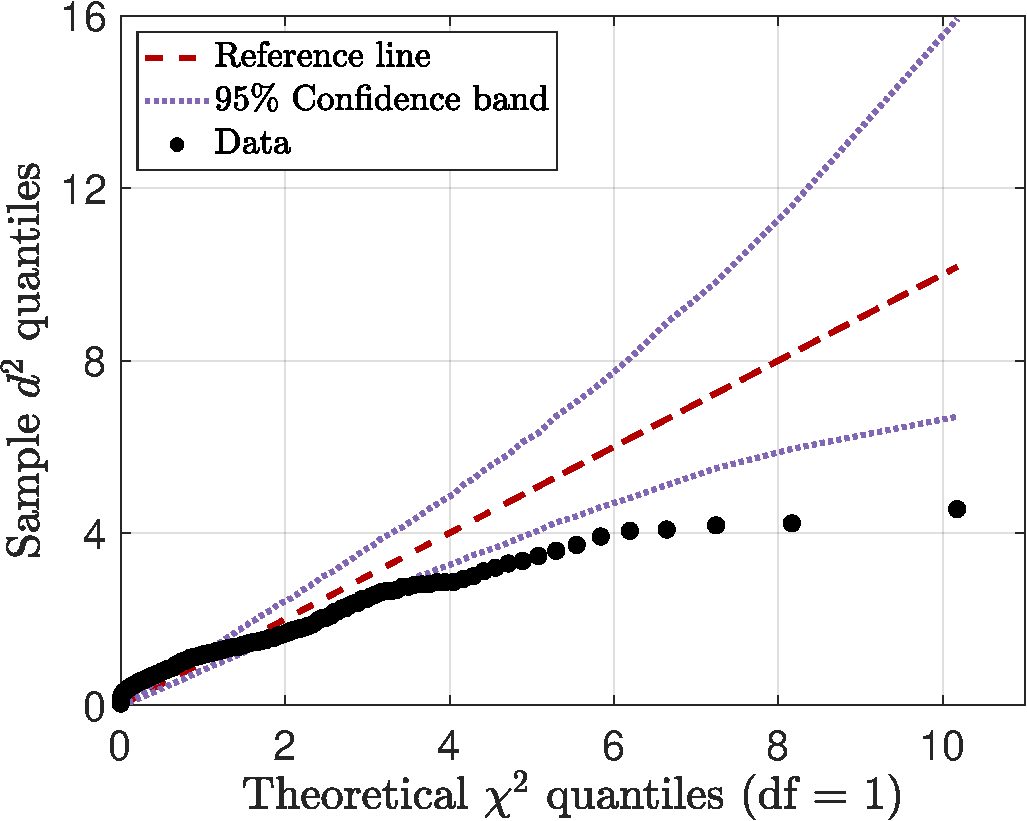
\includegraphics[height=0.36\linewidth]{./figures/test_normal.pdf}&
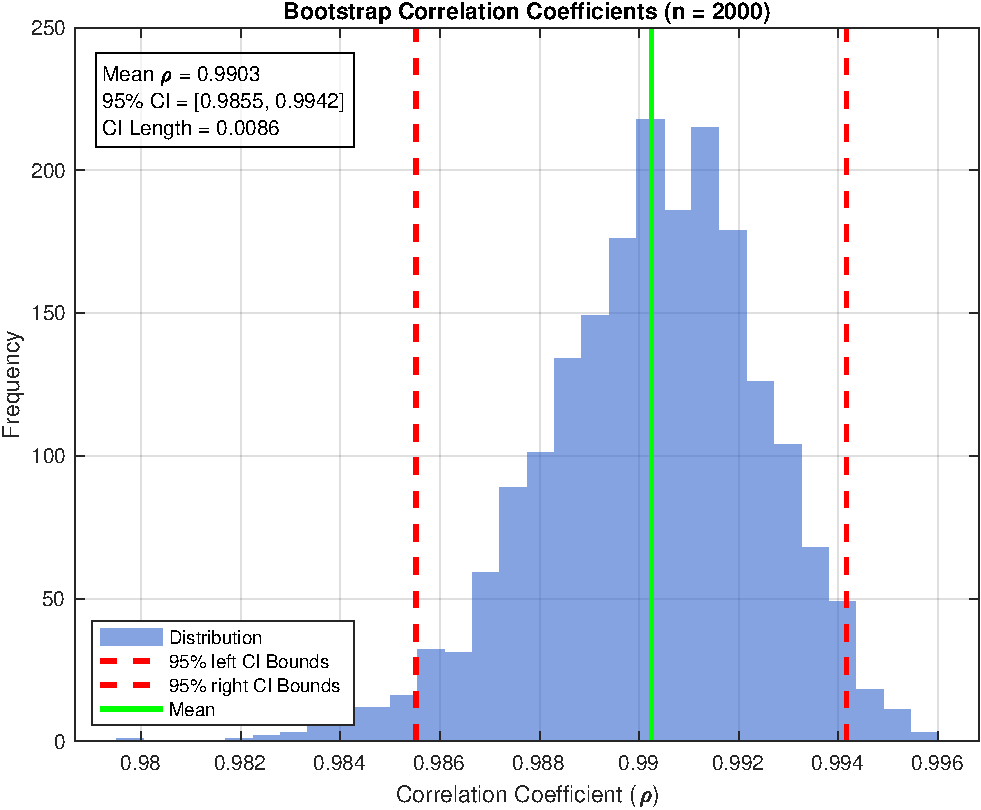
\includegraphics[height=0.36\linewidth]{./figures/CI_bootstrap.pdf}
\end{tabular}
\caption{Left: Quantile-quantile plot of squared Mahalanobis distances versus $\chi^2(1)$ (400 samples, reference mesh). Dashed lines show 95\% bootstrap confidence bands (1000 resamples). Right: Bootstrap confidence intervals for correlation (50 samples, 2000 resamples).}
\label{fig:Test_normal}
\end{figure}
%

Algorithm~\ref{algo:Parameter_Estimation} computes pairwise correlations $\rho_{1,k}$ using statistically independent sample sets, requiring $KQ$ high-fidelity evaluations for $K$ models with $Q$ pilot samples. Cost quantification under $\delta=10\%$ confidence width with $z_{\alpha/2}=1.96$ (95\% confidence) is detailed in Table~\ref{Tab:Offline_cost}. The bootstrap validation in the right plot of Figure \ref{fig:Test_normal} confirms estimator consistency, with bootstrap mean 0.9979 closely aligning with sample correlation 0.9975 despite non-Gaussian distributions. 




The resulting sampling cost efficiencies $\xi$ computed via \eqref{eq:MFMC_sampling_cost_efficiency} exhibit remarkable agreement across spatial resolutions $L=2,\dots,5$
%
\begin{alignat*}{2}
    &\text{Fixed-sample:}\quad &\xi = 8.85\times 10^{-3}, 2.76\times 10^{-3}, 7.70\times 10^{-4}, 5.93\times 10^{-4},\\
    &\text{Dynamic:}\quad &\xi =8.81\times 10^{-3}, 2.65\times 10^{-3}, 7.22\times 10^{-4},  5.97\times 10^{-4}.
\end{alignat*}
%
with maximal deviations under $5\%$. Estimation of theoretical constants $A$ from \eqref{eq:delta_xi_bound} ($A=2.69,2.68,2.53,2.22$ for increasing $L$) overestimate actual $\xi$ variations -- dynamic and fixed estimates differ by $<0.01$ -- demonstrating that dynamic sampling achieves benchmark accuracy at substantially reduced computational cost.








%
\begin{table}[ht]
\centering
\scalebox{0.8}{
\begin{tabular}{|c|c|c|c|c|c|c|c|c|c|c|c|c|c|c|c|c|c|c|}
\hline
\multicolumn{8}{|c|}{Dynamic sampling ($\delta=10\%$ confidence width)} \\
\cline{1-8}	
\multirow{2}{*}{$\epsilon$}&\multicolumn{1}{|c|}{Spatial grid level $\ell$} &0&1&2&3&4&5\\
\cline{2-8}	
&\multicolumn{1}{|c|}{\# of spatial grid nodes $M_\ell$} &$2685$ &$8019$ &$30449$ &$120697$ &$484080$ &$1934365$\\
\hline
\multirow{1}{*}{$[6,8]\times 10^{-3}$} 
&\multicolumn{1}{|c|}{$\rho_{1,k}$}&0.97892&0.99751&1&\multicolumn{3}{c|}{}\\
% &\multicolumn{1}{|c|}{Candidate model $k$} &$\widehat u_{h,3}$&$\widehat u_{h,2}$&$\widehat u_{h,1}$&\multirow{3}{*}{}&\multirow{3}{*}{}&\multirow{3}{*}{}\\
\cline{2-5}		
% &\multicolumn{1}{|c|}{$\sigma_{k}$}&9.7398e-03  &1.2180e-02 &1.1058e-02&&&\\
% \cline{2-5}	
% &\multicolumn{1}{|c|}{$\text{Cov}\left(\widehat u_{h,1},\widehat u_{h,k}\right)$}&1.0368e-04&1.3773e-04 &-&&&\\
% \cline{2-5}
% \hline
% &\multicolumn{1}{|c|}{Sample no. and time}&50&1.6612e+02\\
% \hline
% &\multicolumn{1}{|c|}{$\xi$}&8.81e-03\\
\hline
\multirow{1}{*}{$[2,4]\times 10^{-3}$} 
&\multicolumn{1}{|c|}{$\rho_{1,k}$}&0.98352&0.99660&0.99938&1&\multicolumn{2}{c|}{}\\
\cline{2-6}	
% &\multicolumn{1}{|c|}{Candidate model $k$} &$\widehat u_{h,4}$&$\widehat u_{h,3}$&$\widehat u_{h,2}$&$\widehat u_{h,1}$&\multirow{3}{*}{}&\multirow{3}{*}{}\\
% \cline{2-6}		
% &\multicolumn{1}{|c|}{$\sigma_{k}$}&9.5275e-03&1.2174e-02&9.1390e-03&1.0404e-02&&\\
% \cline{2-6}	
% &\multicolumn{1}{|c|}{$\text{Cov}\left(\widehat u_{h,1},\widehat u_{h,k}\right)$} &1.0227e-04&1.3680e-04 &8.2654e-05&- &&\\

% \hline
% &\multicolumn{1}{|c|}{Sample no. and time}&30&4.5414e+02\\
% \hline
% &\multicolumn{1}{|c|}{$\xi$}&2.65e-03\\
\hline
% \multirow{2}{*}{$4\times 10^{-4}\;\;\sim \;\;1\times 10^{-3}$} &\multicolumn{1}{|c|}{Candidate model $k$} &$\widehat u_{h,5}$&$\widehat u_{h,4}$&$\widehat u_{h,3}$&$\widehat u_{h,2}$&$\widehat u_{h,1}$&\multirow{3}{*}{}\\
%  \cline{2-7}	
% &\multicolumn{1}{|c|}{$\sigma_{k}$}&9.7260e-03&1.2496e-02&1.2300e-02&1.1717e-02&1.1606e-02  &\\
% \cline{2-7}	
% &\multicolumn{1}{|c|}{$\text{Cov}\left(\widehat u_{h,1},\widehat u_{h,k}\right)$}&1.0487e-04&1.4379e-04&1.4983e-04&1.3733e-04  &- &\\
\cline{2-7}	
\multirow{1}{*}{$[0.4, 1]\times 10^{-3}$}&\multicolumn{1}{|c|}{$\rho_{1,k}$}&0.98288&0.99682&0.99941  &0.99976&1 &\\
% \hline
% &\multicolumn{1}{|c|}{Sample no. and time}&50&3.8655e+03\\
% \hline
% &\multicolumn{1}{|c|}{$\xi$}&7.22e-04\\
\hline
% \multirow{2}{*}{$2\times 10^{-4}$} &\multicolumn{1}{|c|}{Candidate model $k$} &$\widehat u_{h,6}$&$\widehat u_{h,5}$&$\widehat u_{h,4}$&$\widehat u_{h,3}$&$\widehat u_{h,2}$&$\widehat u_{h,1}$\\
% \cline{2-8}
% &\multicolumn{1}{|c|}{$\sigma_{k}$}&9.3878e-03&1.0134e-02&1.3305e-02&9.4344e-03&9.7624e-03&1.0524e-02\\
% \cline{2-8}	
% &\multicolumn{1}{|c|}{$\text{Cov}\left(\widehat u_{h,1},\widehat u_{h,k}\right)$}&1.0164e-04&1.0662e-04&1.1679e-04&1.1589e-04&1.0646e-04&-\\
\cline{2-8}	
\multirow{1}{*}{$2\times 10^{-4}$}&\multicolumn{1}{|c|}{$\rho_{1,k}$}&0.98044&0.99787&0.99960&0.99975&0.99970   &1\\
% \hline
% &\multicolumn{1}{|c|}{Sample no. and time}&30&1.2147e+04\\
% \hline
% &\multicolumn{1}{|c|}{$\xi$}&5.97e-04\\
\hline
\multicolumn{8}{|c|}{Benchmark sampling (500 samples)} \\
\hline
% \multirow{2}{*}{$6\times 10^{-3}\;\;\sim \;\;8\times 10^{-3}$} &\multicolumn{1}{|c|}{Candidate model $k$} &$\widehat u_{h,3}$&$\widehat u_{h,2}$&$\widehat u_{h,1}$&\multirow{3}{*}{}&\multirow{3}{*}{}&\multirow{3}{*}{}\\
% \cline{2-5}		
% &\multicolumn{1}{|c|}{$\sigma_{k}$}&9.5720e-03   &1.1549e-02   &1.0939e-02&&&\\
% \cline{2-5}	
% &\multicolumn{1}{|c|}{$\text{Cov}\left(\widehat u_{h,1},\widehat u_{h,k}\right)$}&1.0286e-04&1.2604e-04&-&&&\\
% \cline{2-5}
\multirow{1}{*}{$[6, 8]\times 10^{-3}$}&\multicolumn{1}{|c|}{$\rho_{1,k}$}&0.98238&0.99762&1&\multicolumn{3}{c|}{}\\
% \hline
% &\multicolumn{1}{|c|}{$\xi$}&8.8504e-03\\
\hline
% \multirow{2}{*}{$2\times 10^{-3}\;\;\sim \;\;4\times 10^{-3}$} &\multicolumn{1}{|c|}{Candidate model $k$} &$\widehat u_{h,4}$&$\widehat u_{h,3}$&$\widehat u_{h,2}$&$\widehat u_{h,1}$&\multirow{3}{*}{}&\multirow{3}{*}{}\\
% \cline{2-6}	
% &\multicolumn{1}{|c|}{$\sigma_{k}$}&9.5720e-03   &1.1549e-02   &1.1001e-02   &1.0836e-02 &&\\
% \cline{2-6}	
% &\multicolumn{1}{|c|}{$\text{Cov}\left(\widehat u_{h,1},\widehat u_{h,k}\right)$} &1.0206e-04 &1.2480e-04 &1.1911e-04 &- &&\\
% \cline{2-6}	
\multirow{1}{*}{$[2,4]\times 10^{-3}$}&\multicolumn{1}{|c|}{$\rho_{1,k}$}&0.98394&0.99720 &0.99919&1&\multicolumn{2}{c|}{}\\
% \hline
% &\multicolumn{1}{|c|}{$\xi$}&2.7609e-03\\
\hline
% \multirow{2}{*}{$4\times 10^{-4}\;\;\sim \;\;1\times 10^{-3}$} &\multicolumn{1}{|c|}{Candidate model $k$} &$\widehat u_{h,5}$&$\widehat u_{h,4}$&$\widehat u_{h,3}$&$\widehat u_{h,2}$&$\widehat u_{h,1}$&\multirow{3}{*}{}\\
%  \cline{2-7}	
% &\multicolumn{1}{|c|}{$\sigma_{k}$}&9.5720e-03   &1.1549e-02   &1.1001e-02   &1.0838e-02   &1.0840e-02  &\\
% \cline{2-7}	
% &\multicolumn{1}{|c|}{$\text{Cov}\left(\widehat u_{h,1},\widehat u_{h,k}\right)$}&1.0209e-04 &1.2485e-04 &1.1916e-04 &1.1745e-04 &- &\\
% \cline{2-7}	
\multirow{1}{*}{$[0.4,1]\times 10^{-3}$} &\multicolumn{1}{|c|}{$\rho_{1,k}$}&0.98392 &0.99727 &0.99925 &0.99977&1 &\\
% \hline
% &\multicolumn{1}{|c|}{$\xi$}&7.7012e-04\\
\hline
% \multirow{2}{*}{$2\times 10^{-4}$} &\multicolumn{1}{|c|}{Candidate model $k$} &$\widehat u_{h,6}$&$\widehat u_{h,5}$&$\widehat u_{h,4}$&$\widehat u_{h,3}$&$\widehat u_{h,2}$&$\widehat u_{h,1}$\\
% \cline{2-8}
% &\multicolumn{1}{|c|}{$\sigma_{k}$}&9.5720e-03   &1.1549e-02   &1.1001e-02   &1.0838e-02   &1.0812e-02  &1.0840e-02\\
% \cline{2-8}	
% &\multicolumn{1}{|c|}{$\text{Cov}\left(\widehat u_{h,1},\widehat u_{h,k}\right)$}&1.0209e-04&1.2485e-04&1.1916e-04&1.1745e-04&1.1717e-04&-\\
% \cline{2-8}	
\multirow{1}{*}{$2\times 10^{-4}$}&\multicolumn{1}{|c|}{$\rho_{1,k}$}&0.98390   &0.99728   &0.99925   &0.99977   &0.99976   &1\\
% \hline
% &\multicolumn{1}{|c|}{$\xi$}&5.9298e-04\\
\hline
\end{tabular}}
\caption{Correlation coefficients estimates $\widehat{\rho}_{1,k}$ between high-fidelity model $u_{h,1}$ (spatial level $L$) and candidate low-fidelity models $u_{h,k}$ (sparse grid level $q=1$ on coarser meshes) across tolerance ranges $\epsilon$, with model indices $k = K - \ell$. Top: Dynamic estimation with $\delta=10\%$ confidence width and sample sizes $N_\ell$ from Table~\ref{Tab:Offline_cost}. Bottom: Fixed 500-sample benchmark.}
\label{Tab:MFMC_parameters}
\end{table}
%



% %
% \begin{table}[ht]
% \centering
% \scalebox{0.8}{
% \begin{tabular}{|c|c|c|c|c|c|c|c|c|c|c|c|c|c|c|c|c|c|c|}
% \cline{1-8}	
% \multirow{2}{*}{$\epsilon$}&\multicolumn{1}{|c|}{$\ell$} &0&1&2&3&4&5\\
% \cline{2-8}	
% &\multicolumn{1}{|c|}{$M_\ell$} &$2685$ &$8019$ &$30449$ &$120697$ &$484080$ &$1934365$\\
% \hline
% \multirow{2}{*}{$6\times 10^{-3}\;\;\sim \;\;8\times 10^{-3}$} &\multicolumn{1}{|c|}{Candidate model $k$} &$\widehat u_{h,3}$&$\widehat u_{h,2}$&$\widehat u_{h,1}$&\multirow{3}{*}{}&\multirow{3}{*}{}&\multirow{3}{*}{}\\
% % \cline{2-5}		
% % &\multicolumn{1}{|c|}{$\sigma_{k}$}&9.5720e-03   &1.1549e-02   &1.0939e-02&&&\\
% % \cline{2-5}	
% % &\multicolumn{1}{|c|}{$\text{Cov}\left(\widehat u_{h,1},\widehat u_{h,k}\right)$}&1.0286e-04&1.2604e-04&-&&&\\
% \cline{2-5}
% &\multicolumn{1}{|c|}{$\rho_{1,k}$}&9.8238e-01&9.9762e-01&-&&&\\
% % \hline
% % &\multicolumn{1}{|c|}{$\xi$}&8.8504e-03\\
% \hline
% \multirow{2}{*}{$2\times 10^{-3}\;\;\sim \;\;4\times 10^{-3}$} &\multicolumn{1}{|c|}{Candidate model $k$} &$\widehat u_{h,4}$&$\widehat u_{h,3}$&$\widehat u_{h,2}$&$\widehat u_{h,1}$&\multirow{3}{*}{}&\multirow{3}{*}{}\\
% % \cline{2-6}	
% % &\multicolumn{1}{|c|}{$\sigma_{k}$}&9.5720e-03   &1.1549e-02   &1.1001e-02   &1.0836e-02 &&\\
% % \cline{2-6}	
% % &\multicolumn{1}{|c|}{$\text{Cov}\left(\widehat u_{h,1},\widehat u_{h,k}\right)$} &1.0206e-04 &1.2480e-04 &1.1911e-04 &- &&\\
% \cline{2-6}	
% &\multicolumn{1}{|c|}{$\rho_{1,k}$}&9.8394e-01&9.9720e-01 &9.9919e-01&-&&\\
% % \hline
% % &\multicolumn{1}{|c|}{$\xi$}&2.7609e-03\\
% \hline
% \multirow{2}{*}{$4\times 10^{-4}\;\;\sim \;\;1\times 10^{-3}$} &\multicolumn{1}{|c|}{Candidate model $k$} &$\widehat u_{h,5}$&$\widehat u_{h,4}$&$\widehat u_{h,3}$&$\widehat u_{h,2}$&$\widehat u_{h,1}$&\multirow{3}{*}{}\\
% %  \cline{2-7}	
% % &\multicolumn{1}{|c|}{$\sigma_{k}$}&9.5720e-03   &1.1549e-02   &1.1001e-02   &1.0838e-02   &1.0840e-02  &\\
% % \cline{2-7}	
% % &\multicolumn{1}{|c|}{$\text{Cov}\left(\widehat u_{h,1},\widehat u_{h,k}\right)$}&1.0209e-04 &1.2485e-04 &1.1916e-04 &1.1745e-04 &- &\\
% \cline{2-7}	
% &\multicolumn{1}{|c|}{$\rho_{1,k}$}&9.8392e-01 &9.9727e-01 &9.9925e-01 &9.9977e-01 &- &\\
% % \hline
% % &\multicolumn{1}{|c|}{$\xi$}&7.7012e-04\\
% \hline
% \multirow{2}{*}{$2\times 10^{-4}$} &\multicolumn{1}{|c|}{Candidate model $k$} &$\widehat u_{h,6}$&$\widehat u_{h,5}$&$\widehat u_{h,4}$&$\widehat u_{h,3}$&$\widehat u_{h,2}$&$\widehat u_{h,1}$\\
% % \cline{2-8}
% % &\multicolumn{1}{|c|}{$\sigma_{k}$}&9.5720e-03   &1.1549e-02   &1.1001e-02   &1.0838e-02   &1.0812e-02  &1.0840e-02\\
% % \cline{2-8}	
% % &\multicolumn{1}{|c|}{$\text{Cov}\left(\widehat u_{h,1},\widehat u_{h,k}\right)$}&1.0209e-04&1.2485e-04&1.1916e-04&1.1745e-04&1.1717e-04&-\\
% \cline{2-8}	
% &\multicolumn{1}{|c|}{$\rho_{1,k}$}&9.8390e-01   &9.9728e-01   &9.9925e-01   &9.9977e-01   &9.9976e-01   &-\\
% % \hline
% % &\multicolumn{1}{|c|}{$\xi$}&5.9298e-04\\
% \hline
% \end{tabular}}
% \caption{Estimated statistical parameters for various predetermined tolerances $\epsilon$ in terms of nMSE with 500 samples for approximating parameters between each low fidelity models and the corresponding high fidelity model. The high-fidelity model $\widehat u_{h,1}$ represents the finite element solution to the free boundary problem on a spatial grid of level $L$, ensuring the discretization error meets accuracy requirements. Candidate low-fidelity models $\widehat u_{h,k}$ for $k \geq 2$ are generated using 25 sparse grid nodes (with level $q=1$) on spatial grids from levels 0 to $L-1$. All parameters are estimated using Welford's dynamic sampling algorithm with a stopping criterion requiring a relative error of $10^{-4}$ for all parameters.}
% \label{Tab:MFMC_parameters}
% \end{table}
% %
Building upon the fixed-sample configuration ($\epsilon=2\times10^{-4}$, $Q=500$) in Table~\ref{Tab:MFMC_parameters}, we quantify the evaluation costs per sample for high-fidelity ($W_\ell$) and low-fidelity ($W_\ell^e$) models at spatial levels $\ell=0$ to $5$ through the left plot of Figure~\ref{fig:CostEstimatePlot}. The initial MFMC cost assignments follow $C_1 = W_L$ (high-fidelity) and $C_k = W_{L-k+1}^e$ (low-fidelity). These assignments undergo selective procedure through Algorithm~\ref{algo:enhanced_mfmc_selection}, which enforces parametric conditions of correlation monotonicity and strict cost hierarchy. The observed non-monotonic correlation sequence $|\rho_{1,2}| < |\rho_{1,3}|$ for $\epsilon=2\times10^{-4}$ violates condition (i) of Theorem \ref{thm:Sample_size_est}, requiring the exclusion of $u_{h,2}$ despite its competitive nominal cost. 


% %
% \begin{table}[ht]
% \centering
% \scalebox{0.8}{
% \begin{tabular}{c|c|c|c|c|c|c|c|c|c|c|c|c|c|c|c|c|c|c|}
% \cline{1-7}	
% \multicolumn{1}{|c|}{$\ell$} &0&1&2&3&4&5\\
% \hline
% \multicolumn{1}{|c|}{$M_\ell$} &$2685$ &$8019$ &$30449$ &$120697$ &$484080$ &$1934365$\\
% % \hline
% % \multicolumn{1}{|c|}{Model $k$} &$f_1$&$f_2$&$f_3$&$f_4$&$f_5$&$f_6$\\
% \hline
% \multicolumn{1}{|c|}{$W_\ell$ direct solve}&4.88e-02 &1.49e-01 &6.33e-01 &3.23e+00 &1.55e+01 &7.30e+01\\
% \hline
% \multicolumn{1}{|c|}{$W_\ell^e$ surrog evaluation}&2.68e-04   &5.06e-04   &1.40e-03   &7.03e-03   &2.17e-02   &9.71e-02\\
% \hline
% % \multicolumn{1}{|c|}{$C_\ell$ surrog evaluation( nodes)-source term}&\\
% % \hline
% \end{tabular}}
% \caption{The number of spatial grid points $M_\ell$, cost per sample for both direct computation $W_\ell$ and surrogate evaluation $W_\ell^e$ at an increasing spatial grid level $\ell = 0$ to 5.}
% % and surrogate evaluation with level $q=1$ sparse grid nodes ($P=$)  in the source term.}
% \label{Tab:Dof}
% \end{table}
% %

%
\begin{figure}[ht!]\centering
\begin{tabular}{cc}
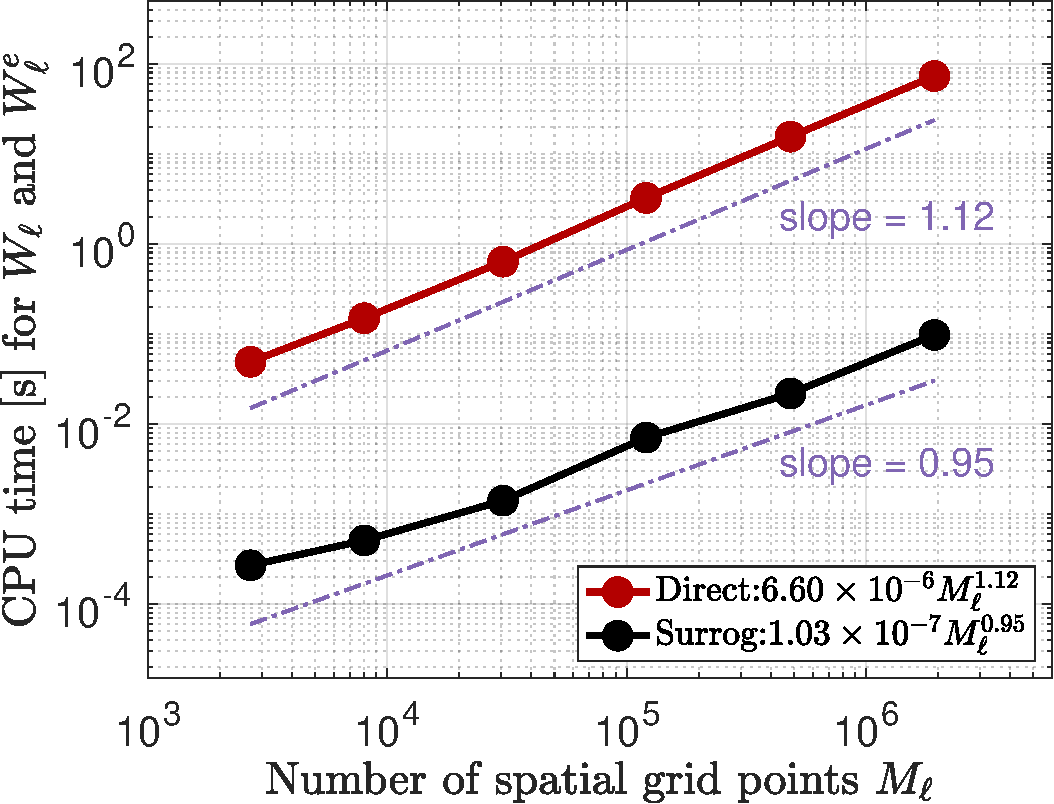
\includegraphics[height=0.36\linewidth]{./figures/CostPerSample_Ml.pdf}&
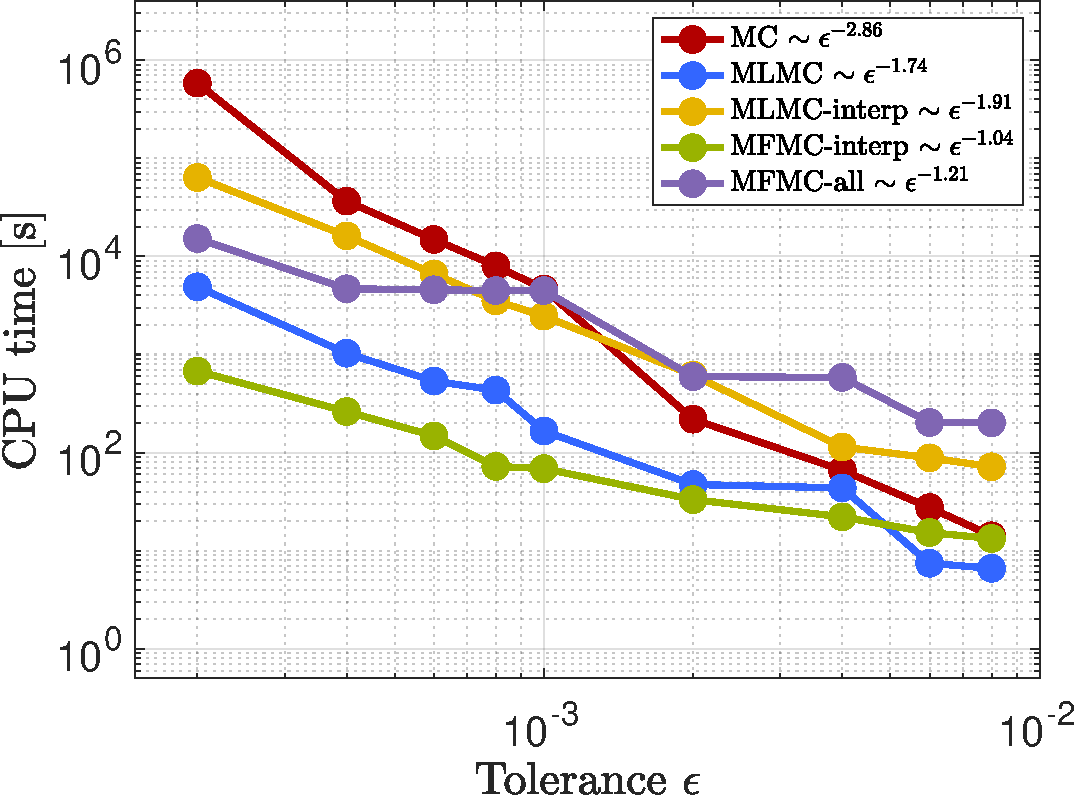
\includegraphics[height=0.36\linewidth]{./figures/Cost_epsilon.pdf}
\end{tabular}
\caption{Left: Mean CPU times of 500 realizations for direct computations $W_\ell$ and surrogate evaluations $W_\ell^e$ versus the number of spatial grid points $M_\ell$ for $\ell = 0$ to 5. Right: Total CPU time versus $\epsilon$ for different simulation methods.}
\label{fig:CostEstimatePlot}
\end{figure}
%




 
 % While the offline preparation incurs non-negligible computational expenses, these costs are justified by the substantial savings achieved during large-scale online sampling, particularly in applications requiring thousands of high-fidelity model evaluations. As a one-time expense, the precomputed surrogates and statistical parameters are reused throughout the online phase, amortizing the initial overhead across all subsequent multi-fidelity Monte Carlo realizations.







% %
% \begin{table}[ht]
% \centering
% \scalebox{0.8}{
% \begin{tabular}{c|c|c|c|c|c|c|c|c|c|c|c|c|c|c|c|c|c|c|}
% \cline{1-7}	
% \multicolumn{1}{|c|}{$\ell$} &0&1&2&3&4&5\\
% \hline
% \multicolumn{1}{|c|}{$M_\ell$} &$2685$ &$8019$ &$30449$ &$120697$ &$484080$ &$1934365$\\
% \hline
% \multicolumn{1}{|c|}{Model $k$} &$\widehat u_{h,5}$&$\widehat u_{h,4}$&$\widehat u_{h,3}$&$\widehat u_{h,2}$&&\\
% \hline
% \multicolumn{1}{|c|}{$\rho_{1,k}$ (24 nodes), ref l=3}&0.9802&0.9958 &0.9976&0.9984&&\\
% \hline
% \multicolumn{1}{|c|}{$\sigma_{k}$}&9.3826e-05 &1.374e-04 &1.2405e-04 &1.2016e-04 &&\\
% \hline
% \multicolumn{1}{|c|}{Covariance} &1.0807e-04 &1.3283e-04 &1.2646e-04 &1.2457e-04 &&\\
% \hline
% \end{tabular}}
% \caption{$\epsilon = 4\times 10^{-3}\;\;\& \;\;2\times 10^{-3}$. High fidelity model: finite element solution on mesh with 120697 grid nodes. $\sigma_1 = 1.2955e-04$. The data are estimated using 500 samples. The selected models are $[\widehat u_{h,2},\widehat u_{h,4},\widehat u_{h,5}]$.}
% % \label{Tab:Dof}
% \end{table}
% %

% %
% \begin{table}[ht]
% \centering
% \scalebox{0.8}{
% \begin{tabular}{c|c|c|c|c|c|c|c|c|c|c|c|c|c|c|c|c|c|c|}
% \cline{1-7}	
% \multicolumn{1}{|c|}{$\ell$} &0&1&2&3&4&5\\
% \hline
% \multicolumn{1}{|c|}{$M_\ell$} &$2685$ &$8019$ &$30449$ &$120697$ &$484080$ &$1934365$\\
% \hline
% \multicolumn{1}{|c|}{Model $k$} &$\widehat u_{h,6}$&$\widehat u_{h,5}$&$\widehat u_{h,4}$&$\widehat u_{h,3}$&$\widehat u_{h,2}$&\\
% \hline
% \multicolumn{1}{|c|}{$\rho_{1,k}$ (24 nodes), ref l=3}&9.0103e-01 &9.2531e-01 &9.2415e-01 &9.2366e-01 &9.2307e-01 &\\
% \hline
% \multicolumn{1}{|c|}{$\sigma_{k}$}&1.1064e-04 &1.3571e-04 &1.2930e-04 &1.2757e-04  &1.2742e-04  &\\
% \hline
% \multicolumn{1}{|c|}{Covariance}&8.9789e-05 &1.2808e-04 &1.1657e-04 &1.1358e-04 &1.1346e-04 &\\
% \hline
% \end{tabular}}
% \caption{$\epsilon = 1\times 10^{-3}\;\;\& \;\;8\times 10^{-4}\;\;\& \;\;6\times 10^{-4}\;\;\& \;\;4\times 10^{-4}$. High fidelity model: finite element solution on mesh with 484080 grid nodes. $\sigma_1 = 1.6794e-04$. The data are estimated using 500 samples.}
% % \label{Tab:Dof}
% \end{table}
% %





% =============================
\subsection{Sampling (online) cost}
% =============================
The online phase uses pre-selected low-fidelity models and estimated parameters $\rho_{1,k}$ and $\alpha_k$ to compute the MFMC estimator. Unbiasedness fundamentally requires statistical independence between samples used for estimating $\alpha_k$ and those used in online evaluation, as justified by the expectation decomposition $\mathbb{E}[\alpha_k Y_k] = \alpha_k \mathbb{E}[Y_k]$ under $\mathbb{E}[Y_k] = 0$ for $k \geq 2$. When computational constraints require sample reuse – particularly for expensive high-fidelity evaluations – $\alpha_k$ become random variables dependent on the same samples generating $Y_k$. This induces correlation that violates the unbiasedness condition, as $\mathbb{E}(\alpha_k Y_k) = \mathbb{E}(\alpha_k Y_k)-\mathbb{E}(\alpha_k)\mathbb{E}(Y_k) = \text{Cov}(\alpha_k,Y_k)\neq 0$, resulting in $\mathbb{E}(A^{\text{MF}}) \neq \mathbb{E}(Y_1)$. While \cite{KoFaPeDiJeNeBu:2022} demonstrates that such bias may be negligible in practice, MLMC circumvents this issue entirely through its fixed weights $\alpha_k \equiv 1$, which permit sample reuse without compromising unbiasedness.

The right plot of Figure \ref{fig:CostEstimatePlot} shows the online sampling cost for the MFMC estimator, scales as $\epsilon^{-1.09}$, reflecting the dominance of high-fidelity computations. Table~\ref{Tab:MFMC_parameters} quantifies this dominance behavior. At $\epsilon=2\times 10^{-4}$, the high-fidelity cost metric $\sqrt{C_1\Delta_1}\approx 0.191$ dominates the aggregated low-fidelity contribution $\sum_{k=2}^{K^*}\sqrt{C_k\Delta_k}\approx 0.0239$ by nearly an order of magnitude. This cost imbalance establishes $c_1 \gg c_{i_k}$ in Theorem~\ref{thm:Sample_cost_est}, confirming the high-fidelity term governs the asymptotic behavior of $\epsilon^{-2+(\beta-\gamma)/\alpha}$. Furthermore, the near-unity correlation $\rho_{1,2}\approx 1$ indicates that $u_{h,2}$ closely resembles the direct nonlinear solve. Applying the correlation decay model from Lemma 2 in \cite{PeGuWi:2018}, $\rho_{1,\ell}^2 - \rho_{1,\ell-1}^2\simeq M_\ell^{-\beta}$, with $\beta\approx 2$ estimated from MLMC variance decay in \cite{ElLiSa:2023}, and using parameters $\alpha\approx 1$ from \cite{ElLiSa:2023, ElLiSa:2025} and $\gamma\approx 1.1$ from Figure \ref{fig:CostEstimatePlot}, the total MFMC sampling cost scales as $\epsilon^{-2+(2-1.1)/1}=\epsilon^{-1.09}$, which matches empirical observations. For comparison,  Monte Carlo exhibits a theoretical cost scaling of $\epsilon^{-2-\gamma/\alpha}\approx\epsilon^{-3.1}$ with observed $\epsilon^{-2.93}$, while multilevel Monte Carlo follows $\epsilon^{-2}$ with observed $\epsilon^{-1.99}$. These results demonstrate exceptional alignment between theoretical cost and empirical measurements across all methods.




The comprehensive cost analysis in Figure~\ref{fig:CostEstimatePlot} reveals insights into multifidelity efficiency when accounting for practical implementation constraints. The yellow dotted curve represents the total MFMC cost (online + offline), where correction terms $Y_k$ from estimator \eqref{eq:MFMC_estimator_Correction} undergo interpolation to a common fine grid to mitigate extrapolation errors inherent in non-nested, geometry-conforming meshes. The analogous MLMC interpolation approach (blue dotted curve) demonstrates comparable mesh-handling requirements. For $\epsilon > 10^{-3}$, MFMC incurs higher computational costs than both Monte Carlo and interpolated MLMC due to offline parameter estimation overhead. However, as $\epsilon$ decreases below $10^{-3}$, MFMC's asymptotic efficiency emerges, ultimately outperforming both MC and MLMC with interpolation. 


Table~\ref{Tab:CPU_time} quantifies this efficiency transition through CPU time measurements and speedup factors relative to Monte Carlo. At $\epsilon=2\times10^{-4}$, MFMC with interpolation achieves 38.4$\times$ speedup while MLMC attains only 9.2$\times$, demonstrating MFMC's superior asymptotic scaling. The theoretical efficiency predicted by \eqref{eq:MFMC_sampling_cost_efficiency} shows minor deviations from empirical speedup metrics due to interpolation overhead, particularly evident at larger $\epsilon$ where fixed computational costs dominate. Notably, including offline costs (rightmost column) significantly impacts efficiency at moderate tolerances but becomes negligible at $\epsilon\leq10^{-3}$, confirming MFMC's suitability for high-precision regimes.


%
\begin{table}[ht]
	\centering
			\scalebox{0.62}{
   \begin{tabular}{c|c|c|c|c|c|c|c|c|c|c|c|c|}
			\hline
			\multicolumn{1}{|c|}{ }&MC-FE &MLMC-FE&MLMC-FE(Interp)
            % &MFMC-FE 
            &MFMC-FE(Interp)&MFMC-FE(Interp)+upfront\\
			\multicolumn{1}{|c|}{$\epsilon$}&Time &\begin{tabular}{cc} \,\,\,\,\,Time & \,\,\,Speedup \end{tabular}&\begin{tabular}{cc} \,\,\,\,Time & \,\,\,Speedup \end{tabular} &\begin{tabular}{cc} \,\,\,\,Time & \,\,\,Speedup \end{tabular} &\begin{tabular}{cc} \,\,\,\,Time & \,\,\,Speedup \end{tabular}\\
            % &\begin{tabular}{cc} \,\,\,\,Time & \,\,\,Speedup \end{tabular}\\
			\hline
			\multicolumn{1}{|c|}{$8\times 10^{-3} $}&1.42e+01&\begin{tabular}{cc}6.61e+00\,\,\, & 2.1 \end{tabular}&\begin{tabular}{cc}7.17e+01\,\,  &0.2\end{tabular}
            % &\begin{tabular}{cc}7.2998e+00\,\,  &1.9453e+00 \end{tabular} 
            &\begin{tabular}{cc}1.33e+01\,\,   &1.1 \end{tabular} &\begin{tabular}{cc}2.01e+02\,\,  &0.07\end{tabular}\\
			\multicolumn{1}{|c|}{$6\times 10^{-3} $}&2.75e+01&\begin{tabular}{cc}7.44e+00\,\,\, & 3.7 \end{tabular}&\begin{tabular}{cc}8.84e+01\,\,  &0.3\end{tabular}
            % &\begin{tabular}{cc}9.3266e+00\,\, &2.9486e+00 \end{tabular}
            &\begin{tabular}{cc}1.53e+01&1.8
            \end{tabular}&\begin{tabular}{cc}2.03e+02\,\,  &0.1\end{tabular}\\
			\multicolumn{1}{|c|}{$4\times 10^{-3} $}&6.60e+01&\begin{tabular}{cc}4.36e+01\,\,\, & 1.5 \end{tabular}&\begin{tabular}{cc}1.14e+02\,\,  &0.6\end{tabular}
            % &\begin{tabular}{cc}1.9119e+01&3.4521e+00\end{tabular}
            &\begin{tabular}{cc}2.21e+01&3.0
            \end{tabular}&\begin{tabular}{cc}5.84e+02\,\,  &0.1\end{tabular}\\
			\multicolumn{1}{|c|}{$2\times 10^{-3} $}&2.19e+02&\begin{tabular}{cc}4.73e+01\,\, & 4.6\end{tabular}&\begin{tabular}{cc}6.16e+02\,\,  &0.4\end{tabular}
            % &\begin{tabular}{cc}3.0242e+01& 7.2416e+00\end{tabular}
            &\begin{tabular}{cc}3.32e+01&6.6 \end{tabular}&\begin{tabular}{cc}5.95e+02\,\,  &0.4\end{tabular}\\
			\multicolumn{1}{|c|}{$10^{-3} $}&4.66e+03&\begin{tabular}{cr}1.66e+02\,\, & 28.1 \end{tabular}&\begin{tabular}{cc}2.46e+03\,\,  &1.9\end{tabular}
            % &\begin{tabular}{cc}6.5732e+01&7.0894e+01\end{tabular}
            &\begin{tabular}{cc}6.87e+01&67.9
            \end{tabular}&\begin{tabular}{cc}4.49e+03\,\,  &1.0\end{tabular}\\
			\multicolumn{1}{|c|}{$8\times 10^{-4} $}&8.02e+03&\begin{tabular}{cc}4.33e+02\,\, & 18.5 \end{tabular}&\begin{tabular}{cc}3.53e+03\,\,  &2.3\end{tabular}
            % &\begin{tabular}{cc}6.9345e+01&1.1565e+02\end{tabular}
            &\begin{tabular}{cc}7.23e+01&111.0
            \end{tabular}&\begin{tabular}{cc}4.49e+03\,\,  &1.8\end{tabular}\\
			\multicolumn{1}{|c|}{$6\times 10^{-4} $}&1.49e+04&\begin{tabular}{cc}5.36e+02\,\, & 27.8 \end{tabular}&\begin{tabular}{cc}6.63e+03\,\,  &2.2\end{tabular}
            % &\begin{tabular}{cc}1.4482e+02&1.0289e+02\end{tabular}
            &\begin{tabular}{cc}1.48e+02&100.6
            \end{tabular}&\begin{tabular}{cc}4.57e+03\,\,  &3.3\end{tabular}\\
                \multicolumn{1}{|c|}{$4\times 10^{-4} $}&3.66e+04&\begin{tabular}{cc}1.03e+03\,\, & 35.4 \end{tabular}&\begin{tabular}{cc}1.62e+04\,\,  &2.3\end{tabular} &\begin{tabular}{cc}2.62e+02&139.7 \end{tabular}
                % &\begin{tabular}{cc}2.6595e+02&1.3762e+02\end{tabular}
            &\begin{tabular}{cc}4.68e+03\,\,  &7.8\end{tabular}\\
                \multicolumn{1}{|c|}{$2\times 10^{-4} $}&5.84e+05$^{\ast}$\!\!\!&\begin{tabular}{cc}4.90e+03 &119.2 \end{tabular} &\begin{tabular}{cc}6.38e+04\,\,  &9.2\end{tabular}
                % &\begin{tabular}{cc} 6.6985e+02&8.7184e+02 \end{tabular}
                &\begin{tabular}{cc}6.78e+02 &861.2 \end{tabular}&\begin{tabular}{cc}1.52e+04\,\,  &38.4\end{tabular}\\
			\hline
	\end{tabular}
 }
	\caption{CPU time (in seconds) for various simulation methods: Monte Carlo with finite elements (MC-FE), multilevel Monte Carlo with finite elements (MLMC-FE), MLMC-FE with interpolation to a common grid at level $\ell=5$, multifidelity Monte Carlo with finite elements (MFMC-FE) with interpolation to a common grid at level $\ell=5$, and MFMC-FE with interpolation and offline cost inclusion. The table also presents speedup factors for these methods relative to MC-FE at different tolerances $\epsilon$. The CPU time for MC-FE at $\epsilon = 2\times 10^{-4}$ (marked with an asterisk) is an estimate due to prohibitive computational cost.}
	\label{Tab:CPU_time}
\end{table}
%




The efficiency changes stems from MFMC's sample redistribution across fidelity levels, detailed in Table~\ref{Tab:SampleSize}. As $\epsilon$ decreases, all methods increase total samples while refining discretizations, but MFMC dramatically shifts computational burden to low-fidelity models. At $\epsilon=2\times10^{-4}$, MFMC utilizes 97,028 low-fidelity samples compared to MLMC's 15,619 and MC's 8,000, representing 97.1\% versus 93.8\% and 0\% low-fidelity utilization respectively. This redistribution, while increasing absolute sample counts by 6.2 times over MLMC, reduces high-fidelity evaluations by 3.7 times, yielding net efficiency gains that increase with precision requirements.




%
\begin{table}[ht]
	\centering
			\scalebox{0.62}{
   \begin{tabular}{c|c|c|c|c|c|c|c|c|c|c|c|c|}
	    \cline{2-7}	
		&\multicolumn{6}{|c|}{ Level $\ell$}\\
			\hline
			\multicolumn{1}{|c|}{$\epsilon$}&0&1&2&3&4&5\\
			\hline
			\multicolumn{1}{|c|}{$8\times 10^{-3} $}&&&5&&&\\
			\multicolumn{1}{|c|}{$6\times 10^{-3} $}&&&9&&&\\
			\multicolumn{1}{|c|}{$4\times 10^{-3} $}&&&&21&&\\
			\multicolumn{1}{|c|}{$2\times 10^{-3} $}&&&&73&&\\
			\multicolumn{1}{|c|}{$10^{-3} $}&&&&&287&\\
			\multicolumn{1}{|c|}{$8\times 10^{-4} $}&&&&&445&\\
			\multicolumn{1}{|c|}{$6\times 10^{-4} $}&&&&&845&\\
                \multicolumn{1}{|c|}{$4\times 10^{-4} $}&&&&&2000&\\
                \multicolumn{1}{|c|}{$2\times 10^{-4} $}&&&&&& 8000$^{\ast}$\!\!\\
			\hline
	\end{tabular}
 \qquad
		\begin{tabular}{c|c|c|c|c|c|c|c|c|c|c|c|c|}
	    \cline{2-7}	
		&\multicolumn{6}{|c|}{ Level $\ell$}\\
			\hline
			\multicolumn{1}{|c|}{$\epsilon$}&0&1&2&3&4&5\\
			\hline
			\multicolumn{1}{|c|}{$8\times 10^{-3} $}&10     &2     &2&&&\\
			\multicolumn{1}{|c|}{$6\times 10^{-3} $}&12     &2     &2&&&\\
			\multicolumn{1}{|c|}{$4\times 10^{-3} $}&22     &5     &2     &2&&\\
			\multicolumn{1}{|c|}{$2\times 10^{-3} $}&163    &26     &5     &2&&\\
			\multicolumn{1}{|c|}{$10^{-3} $}&577   &90    &15     &3     &2&\\
			\multicolumn{1}{|c|}{$8\times 10^{-4} $}&1036 &157 &26 &5 &2&\\
			\multicolumn{1}{|c|}{$6\times 10^{-4} $}&1744 &266 &44 &9 &2&\\
                \multicolumn{1}{|c|}{$4\times 10^{-4} $}&3911 &553 &86 &17 &4&\\
                \multicolumn{1}{|c|}{$2\times 10^{-4} $}&15619 &2298 &370 &57 &12 &2\\
			\hline
	\end{tabular}
 \qquad
		\begin{tabular}{c|c|c|c|c|c|c|c|c|c|c|c|c|c|c|c|c|c|}
	    \cline{2-7}	
		&\multicolumn{6}{|c|}{ Level $\ell$}\\
			\hline
			\multicolumn{1}{|c|}{$\epsilon$}&0&1&2&3&4&5\\
			\hline
			\multicolumn{1}{|c|}{$8\times 10^{-3} $}&24&4&2&&&\\
			\multicolumn{1}{|c|}{$6\times 10^{-3} $}&43&7&2&&&\\
			\multicolumn{1}{|c|}{$4\times 10^{-3} $}&95&12&4&2&&\\
			\multicolumn{1}{|c|}{$2\times 10^{-3} $}&380&46&13&2&&\\
			\multicolumn{1}{|c|}{$10^{-3} $}&2444&301&79&13&2&\\
			\multicolumn{1}{|c|}{$8\times 10^{-4} $}&3819&470&123&21&2&\\
                \multicolumn{1}{|c|}{$6\times 10^{-4} $}&6788&835&218&36&2&\\
			\multicolumn{1}{|c|}{$4\times 10^{-4} $}&15273&1879&489&81&2&\\
                \multicolumn{1}{|c|}{$2\times 10^{-4} $}&97028&13374&2544&335&-&5\\
			\hline
	\end{tabular}
 
 }
	\caption{Optimal sample size estimation for MC-FE (left), MLMC-FE (middle), and MFMC-FE (right) for various tolerance values $\epsilon$. The computational cost for Monte Carlo with a tolerance of $\epsilon = 2\times 10^{-4}$ was prohibitive; therefore, the entry for this tolerance (marked with an asterisk) is an estimate.}
	\label{Tab:SampleSize}
\end{table}
%




% \JLcolor{According to \cite{PeGuWi:2018}, pages A3174 and A3181–A3182, perturbations in the sample variance and sample correlation coefficients have a small impact on the overall sample size and computational work. However, from my perspective, inaccurate estimation of these statistical parameters can also affect the model selection process. If these statistics are not reliably computed, low-fidelity models with misleading characteristics may be selected or rejected incorrectly, potentially undermining the efficiency and accuracy of the MFMC framework. In particular, models that exhibit inconsistent statistical properties violating the two conditions in Theorem \ref{thm:Sample_size_est} could be included, leading to suboptimal model choices for the low-fidelity approximations and, consequently, affecting the overall performance of the multi-fidelity estimator.}






% =============================
\subsection{Properties of plasma boundary and geometric descriptors}
% =============================
Maintaining plasma boundary fidelity presents significant computational challenges in multilevel Monte Carlo frameworks, particularly when aggregating sample corrections across multiple resolution levels. As established in \cite{ElLiSa:2023}, geometric distortions emerge from extrapolation errors during cross-level correction on non-nested, geometry-conforming meshes. These artifacts originate from spatial resolution mismatches when projecting coarse-grid solutions onto finer discretizations, causing topological inconsistencies at critical boundary regions such as the X-point and divertor strike points.


To preserve geometric integrity, we implement a unified interpolation strategy across methodologies: MLMC solutions are interpolated to a reference grid at level $\ell=5$, while MFMC corrections from low-fidelity models -- computed via stochastic collocation on coarse grids -- undergo identical interpolation, achieving comparable geometric consistency.

Visual evidence in Figure \ref{fig:QoI_plot} demonstrates near-identical plasma boundaries across Monte Carlo, interpolated MLMC, and MFMC methods. Quantitative validation in Table \ref{Tab:QoI_GeoInfo} confirms 
exceptional agreement: geometric descriptors for both MLMC and MFMC match the Monte Carlo benchmark within 0.5\% relative error, with all key parameters agreeing to two decimal places. This geometric preservation is crucial for accurate quantification of shape-dependent phenomena. 



%=====================================================================================
% \noindent \textbf{Plasma boundary.} 
%=====================================================================================






% %
% \begin{table}[ht]
% \centering
% \scalebox{0.8}{
% \begin{tabular}{c|c|c|c|c|c|c|c|c|c|c|c|c|c|c|c|c|c|c|}
% \cline{1-7}	
% \multicolumn{1}{|c|}{Dof} &$1934365$&$484080$&$120697$&$30449$&$8019$&$2685$\\
% \hline
% \multicolumn{1}{|c|}{Model $k$} &$f_1$&$f_2$&$f_3$&$f_4$&$f_5$&$f_6$\\
% % \hline
% % \multicolumn{1}{|c|}{$C_k$ direct solve}&1.2029e+02&2.6478e+01&5.3710e+00&1.1269e+00&2.9300e-01&9.6419e-02\\
% % \hline
% % \multicolumn{1}{|c|}{$C_k$ surrog evaluation(24 nodes)}&1.2595e-01&2.9694e-02&9.1085e-03&3.0580e-03&1.1869e-03&2.5127e-04\\
% \hline
% \multicolumn{1}{|c|}{$\rho_{1,k}$ (24 nodes), ref l=3}&&&&0.9678&0.9670&0.9488\\
% \hline
% \multicolumn{1}{|c|}{$\sigma_{k}$}&&&&1.1696e-04&1.2929e-04&8.8977e-05\\
% \hline
% \multicolumn{1}{|c|}{Covariance}&&&&1.3065e-04&1.3726e-04&1.1172e-04\\
% \hline
% \end{tabular}}
% \caption{High fidelity model: finite element solution on mesh with 30449 grid nodes. $\sigma_1 = 1.5582e-04$. The data are estimated using 500 samples.}
% % \label{Tab:Dof}
% \end{table}
% %









   

   


\begin{figure}[ht!]\centering
\begin{tabular}{ccc}
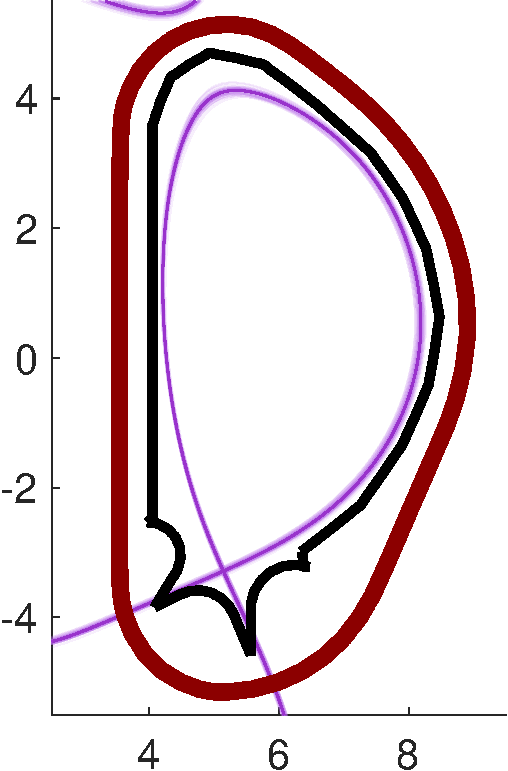
\includegraphics[width=0.19\linewidth]{./figures/QoI_MC_uniform.pdf}
% &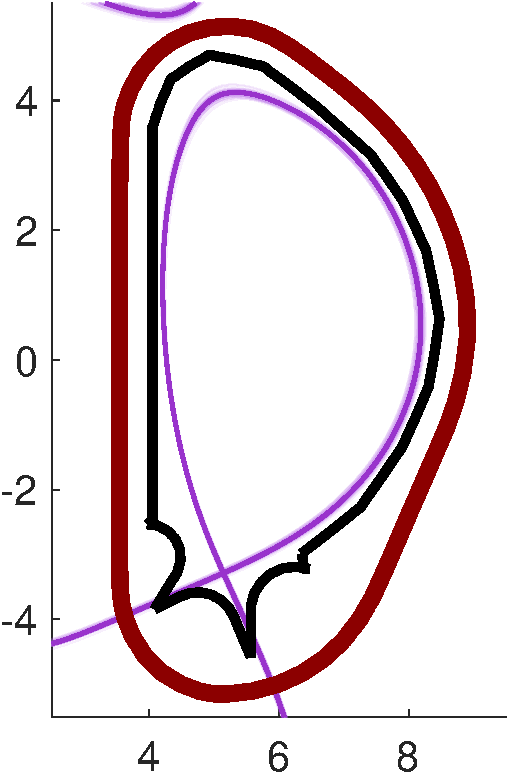
\includegraphics[width=0.19\linewidth]{./figures/QoI_MC_surrogate.pdf}
&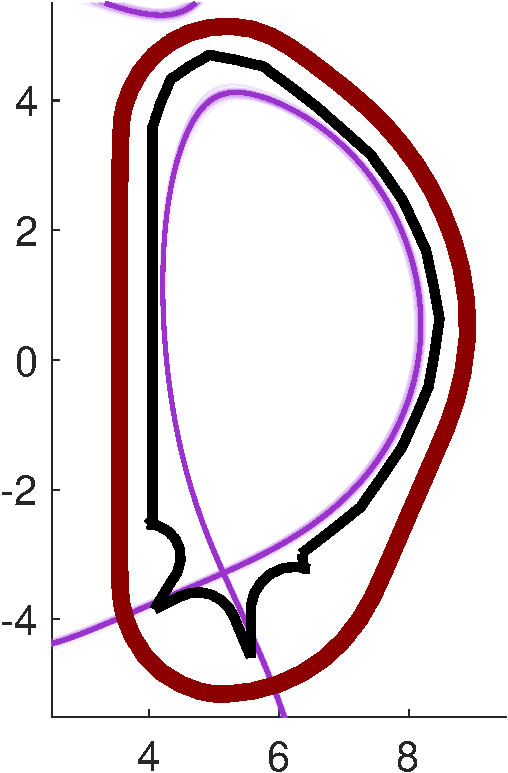
\includegraphics[width=0.19\linewidth]{./figures/QoI_MLMC_DirectSolver_Interp2CommonGrid.pdf} 
& 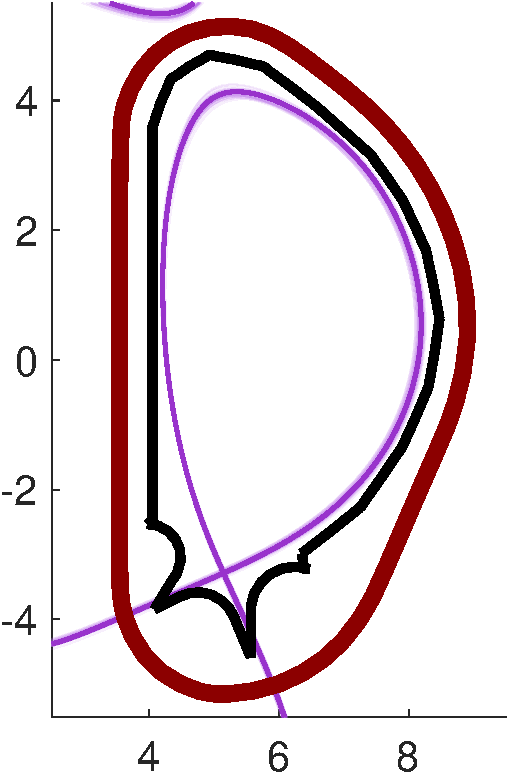
\includegraphics[width=0.19\linewidth]{./figures/QoI_MFMC.pdf} 
\\
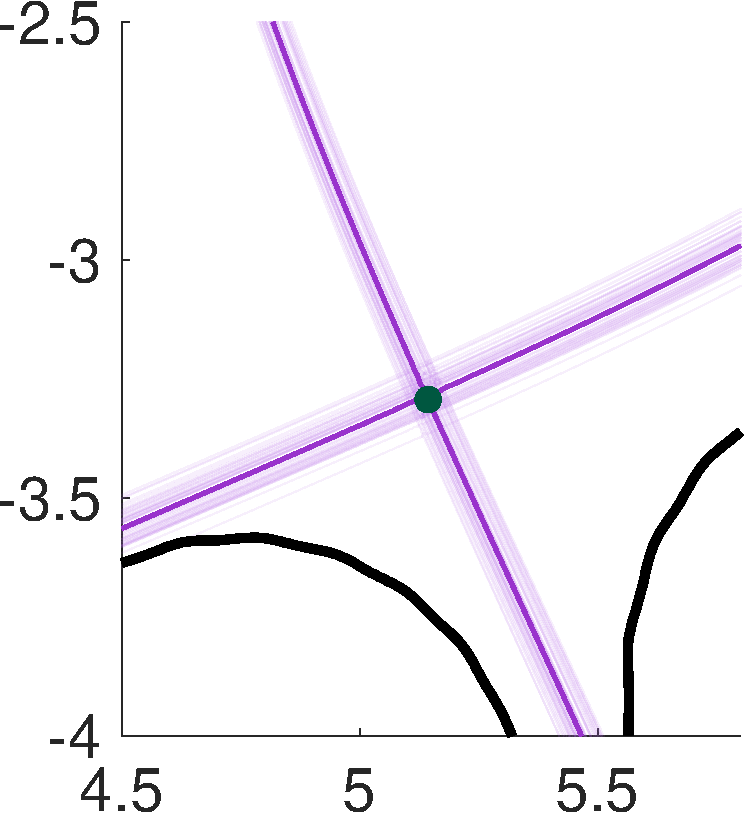
\includegraphics[width=0.19\linewidth]{./figures/QoI_MC_uniform_xptRegion.pdf} 
% &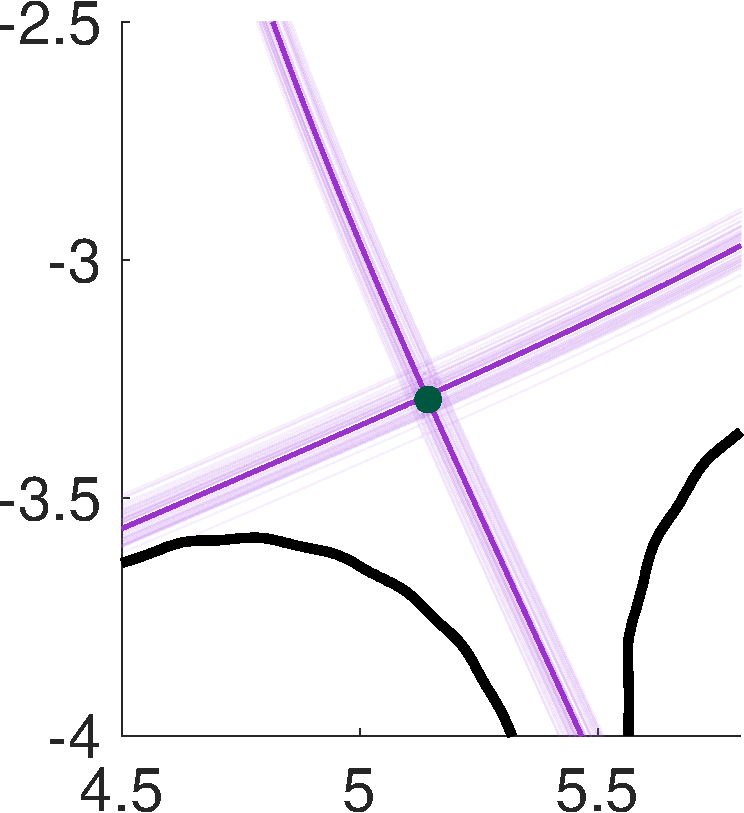
\includegraphics[width=0.19\linewidth]{./figures/QoI_MC_surrogate_xptRegion.pdf}
&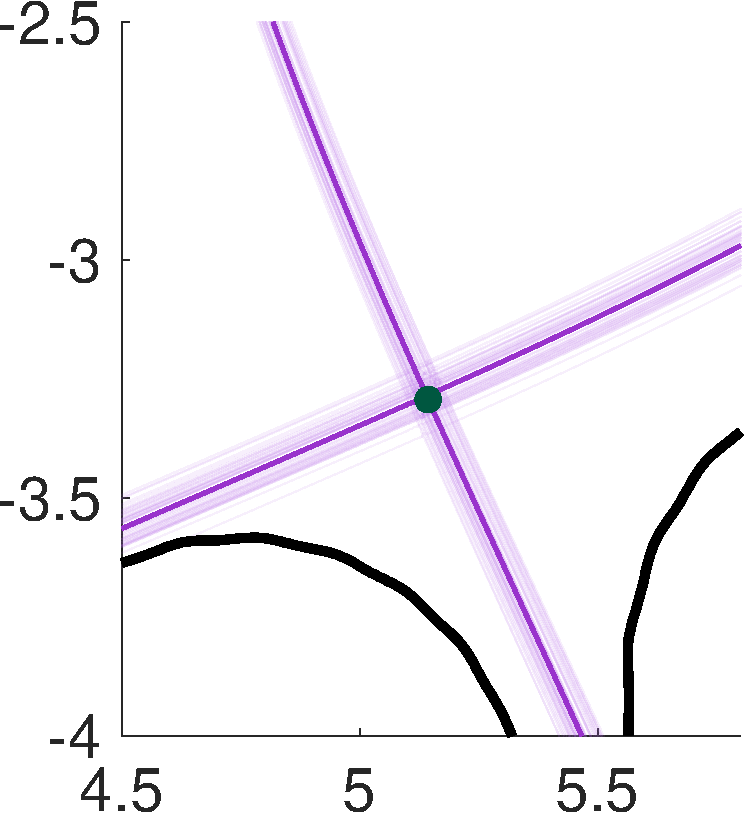
\includegraphics[width=0.19\linewidth]{./figures/QoI_MLMC_DirectSolver_xptRegion_Interp2CommonGrid.pdf} 
&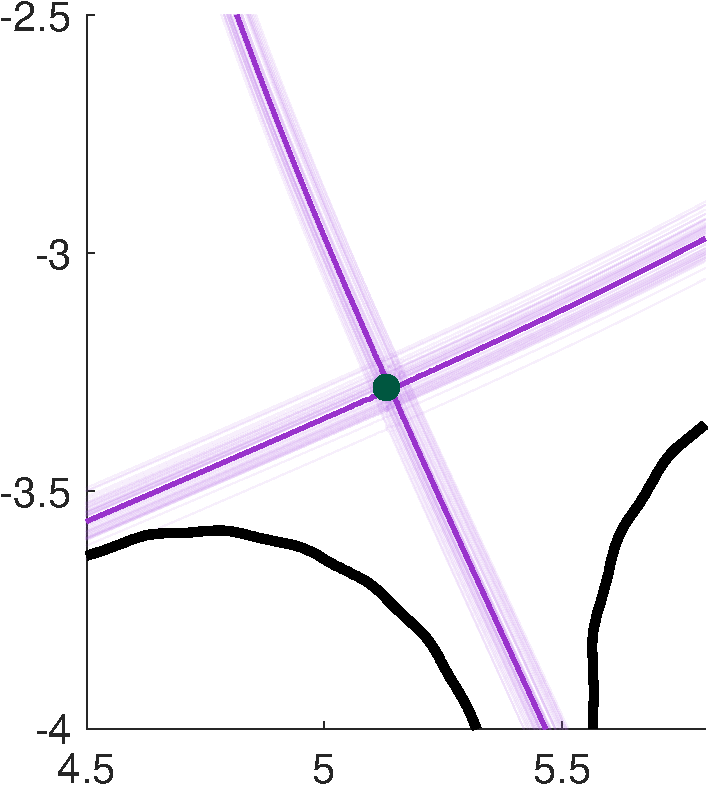
\includegraphics[width=0.19\linewidth]{./figures/QoI_MFMC_xptRegion.pdf} 
\\[1ex]
\quad MC-FE &MLMC-FE (Interp) &MFMC-FE (Interp) \\[-0.5ex]
\end{tabular}
\caption{The plasma boundaries of 50 random realizations are overlaid in the top row as violet curves. The solid violet line represents the plasma boundary of the expected poloidal flux generated with tolerance $\epsilon=4\times 10^{-4}$. The reactor's inner and outer walls are shown in solid black and dark red, respectively. The bottom row provides a detailed view of the regions close to the x-points, with dark green dots indicating the x-points of the expected solution. The columns, from left to right, show the simulations using the MC-FE, MLMC-FE, and MFMC-FE approaches, all interpolated to geometry-conforming uniform meshes at discretization level $\ell=5$.}
\label{fig:QoI_plot}
\end{figure}
%














% \noindent \textbf{Geometric descriptors.}
%
\begin{table}[ht]
	\centering
			\scalebox{0.7}{
		\begin{tabular}{c|c|c|c|c|c|c|}
			\cline{2-5}
				&\multicolumn{1}{c|}{MC-FE}&MLMC-FE&MLMC-FE (Interp)&MFMC-FE (Interp)\\
			\hline
			\multicolumn{1}{|c|}{x point}&(5.14,-3.29)&(5.14,-3.29)&(5.14,-3.29)&(5.14,-3.29)\\
			\hline
			\multicolumn{1}{|c|}{magnetic axis}&(6.41,0.61)&(6.44,0.56)&(6.41,0.61)&(6.41,0.61)\\
			\hline
			\multicolumn{1}{|c|}{strike} &(4.16,-3.71)&(4.16,-3.71)&(4.16,-3.71)&(4.16,-3.71)\\
			\multicolumn{1}{|c|}{points}&(5.56,-4.22)&(5.56,-4.22)&(5.56,-4.22)&(5.56,-4.22)\\
			\hline
			\multicolumn{1}{|c|}{inverse aspect ratio} &0.32&0.32&0.32&0.32\\
			\hline
			\multicolumn{1}{|c|}{elongation} &1.86&1.87&1.86&1.86\\
			\hline
			\multicolumn{1}{|c|}{upper triangularity}&0.43&0.43&0.43&0.43\\
			\hline
			\multicolumn{1}{|c|}{lower triangularity} &0.53&0.53&0.53&0.53\\
			\hline
	\end{tabular}
  }
	\caption{Geometric parameters of the expected poloidal flux $u$ for different simulation methods: MC-FE with direct solver, MLMC-FE with direct solver, MLMC-FE with direct solver and interpolation of the solution to a common fine grid at level $\ell=5$, and MFMC-FE with interpolation of the solution to a common fine grid at level $\ell=5$. The results are generated with an nMSE of $4 \times 10^{-4}$.}
	\label{Tab:QoI_GeoInfo}
\end{table}







% % =============================
% \subsection{Uncertainties in the source term}
% % =============================
% In this experiment, we study the uncertainty in perturbing the reference parameter that characterizes the source term \eqref{eq:source}.
% \begin{table}[ht]
% 	\centering
% 			\scalebox{0.62}{
%    \begin{tabular}{c|c|c|c|c|c|c|c|c|c|c|c|c|}
% 	    \cline{2-7}	
% 		&\multicolumn{6}{|c|}{ Level $\ell$}\\
% 			\hline
% 			\multicolumn{1}{|c|}{$\epsilon$}&0&1&2&3&4&5\\
% 			\hline
% 			\multicolumn{1}{|c|}{$8\times 10^{-3} $}&&&8&&&\\
% 			\multicolumn{1}{|c|}{$6\times 10^{-3} $}&&&10&&&\\
% 			\multicolumn{1}{|c|}{$4\times 10^{-3} $}&&&&25&&\\
% 			\multicolumn{1}{|c|}{$2\times 10^{-3} $}&&&&93&&\\
% 			\multicolumn{1}{|c|}{$10^{-3} $}&&&&&423&\\
% 			\multicolumn{1}{|c|}{$8\times 10^{-4} $}&&&&&678&\\
% 			\multicolumn{1}{|c|}{$6\times 10^{-4} $}&&&&&1211&\\
%                 \multicolumn{1}{|c|}{$4\times 10^{-4} $}&&&&&2700$^{\ast}$&\\
%                 \multicolumn{1}{|c|}{$2\times 10^{-4} $}&&&&&&11000$^{\ast}$\!\!\\
% 			\hline
% 	\end{tabular}
%  \qquad
% 		\begin{tabular}{c|c|c|c|c|c|c|c|c|c|c|c|c|}
% 	    \cline{2-7}	
% 		&\multicolumn{6}{|c|}{ Level $\ell$}\\
% 			\hline
% 			\multicolumn{1}{|c|}{$\epsilon$}&0&1&2&3&4&5\\
% 			\hline
% 			\multicolumn{1}{|c|}{$8\times 10^{-3} $}&10 &2 &2&&&\\
% 			\multicolumn{1}{|c|}{$6\times 10^{-3} $}&11 &3 &2 &&&\\
% 			\multicolumn{1}{|c|}{$4\times 10^{-3} $}&33 &7 &2 &2&&\\
% 			\multicolumn{1}{|c|}{$2\times 10^{-3} $}&150 &27 &4 &2&&\\
% 			\multicolumn{1}{|c|}{$10^{-3} $}&692 &116 &19 &4 &2&\\
% 			\multicolumn{1}{|c|}{$8\times 10^{-4} $}&1008 &160 &27 &6 &2&\\
% 			\multicolumn{1}{|c|}{$6\times 10^{-4} $}&2022 &322 &53 &10 &3&\\
%                 \multicolumn{1}{|c|}{$4\times 10^{-4} $}&4158 &613 &106 &14 &4&\\
%                 \multicolumn{1}{|c|}{$2\times 10^{-4} $}&17158 &2612 &442 &59 &13 &2\\
% 			\hline
% 	\end{tabular}
%  \qquad
% 		\begin{tabular}{c|c|c|c|c|c|c|c|c|c|c|c|c|c|c|c|c|c|}
% 	    \cline{2-7}	
% 		&\multicolumn{6}{|c|}{ Level $\ell$}\\
% 			\hline
% 			\multicolumn{1}{|c|}{$\epsilon$}&0&1&2&3&4&5\\
% 			\hline
% 			\multicolumn{1}{|c|}{$8\times 10^{-3} $}&&&&&&\\
% 			\multicolumn{1}{|c|}{$6\times 10^{-3} $}&&&&&&\\
% 			\multicolumn{1}{|c|}{$4\times 10^{-3} $}&&&\\
% 			\multicolumn{1}{|c|}{$2\times 10^{-3} $}&&&\\
% 			\multicolumn{1}{|c|}{$10^{-3} $}&&&&&&\\
% 			\multicolumn{1}{|c|}{$8\times 10^{-4} $}&&&&&&\\
%                 \multicolumn{1}{|c|}{$6\times 10^{-4} $}&&&&&&\\
% 			\multicolumn{1}{|c|}{$4\times 10^{-4} $}&&&&&&\\
%                 \multicolumn{1}{|c|}{$2\times 10^{-4} $}&&&&&&\\
% 			\hline
% 	\end{tabular}
 
%  }
% 	\caption{The optimal sample size estimation for MC-FE (left), uniform MLMC-FE (middle), and MFMC-FE (right). The simulations were conducted for a variety of choices of $\epsilon$. The computational cost associated with a tolerance of $\epsilon = 2\times 10^{-4}$ for Monte Carlo was prohibitive; the entry in the table for this tolerance (with an asterisk) is an estimate.}
% 	\label{Tab:SampleSize_Source_Term}
% \end{table}

% \begin{table}[ht]
% 	\centering
% 			\scalebox{0.62}{
%    \begin{tabular}{c|c|c|c|c|c|c|c|c|c|c|c|c|}
% 			\hline
% 			\multicolumn{1}{|c|}{ }&MC-FE &MLMC-FE &MFMC-FE\\
% 			\multicolumn{1}{|c|}{$\epsilon$}&Time & \begin{tabular}{cc} \,\,\,\,\,Time & \,\,\,Speedup \end{tabular}  &\begin{tabular}{cc} \,\,\,\,Time & \,\,\,Speedup \end{tabular}\\
% 			\hline
% 			\multicolumn{1}{|c|}{$8\times 10^{-3} $}&9.71e+01&\begin{tabular}{cc}1.10e+01\,\,\, & 8.8 \end{tabular}&\begin{tabular}{cc}..\,\,  & .. \end{tabular} \\
% 			\multicolumn{1}{|c|}{$6\times 10^{-3} $}&1.16e+02&\begin{tabular}{cc}1.27e+01\,\,\, & 9.1 \end{tabular}&\begin{tabular}{cc}..\,\, &.. \end{tabular}\\
% 			\multicolumn{1}{|c|}{$4\times 10^{-3} $}&1.29e+02&\begin{tabular}{cc}3.39e+01\,\,\, & 3.8 \end{tabular}&\begin{tabular}{cc}..& .. \end{tabular}\\
% 			\multicolumn{1}{|c|}{$2\times 10^{-3} $}&8.03e+02&\begin{tabular}{cc}7.29e+01\,\, & 11.0\end{tabular}&\begin{tabular}{cc}..& .. \end{tabular}\\
% 			\multicolumn{1}{|c|}{$10^{-3} $}&1.49e+04&\begin{tabular}{cr}2.55e+02\,\, & 58.5 \end{tabular}&\begin{tabular}{cc}..& .. \end{tabular}\\
% 			\multicolumn{1}{|c|}{$8\times 10^{-4} $}&3.89e+04&\begin{tabular}{cc}2.76e+02\,\, &140.6 \end{tabular}&\begin{tabular}{cc}..& ..
%             \end{tabular}\\
% 			\multicolumn{1}{|c|}{$6\times 10^{-4} $}&1.1219e+05&\begin{tabular}{cc}7.1946e+02\,\, & .. \end{tabular}&\begin{tabular}{cc}.. & .. \end{tabular}\\
%                 \multicolumn{1}{|c|}{$4\times 10^{-4} $}&..&\begin{tabular}{cc}1.1598e+03\,\, & .. \end{tabular} &\begin{tabular}{cc}..& .. \end{tabular}\\
%                 \multicolumn{1}{|c|}{$2\times 10^{-4} $}&..$^{\ast}$\!\!\!&\begin{tabular}{cc}4.4956e+03 &.. \end{tabular} &\begin{tabular}{cc}..&.. \end{tabular}\\
% 			\hline
% 	\end{tabular}
%  }
% 	\caption{The CPU time in seconds for MC-FE (left), uniform MLMC-FE (middle), and MFMC-FE (right), together with speedups for the multilevel methods, for a variety of choices of $\epsilon$. The computational cost associated with a tolerance of $\epsilon = 2\times 10^{-4}$ for Monte Carlo was prohibitive; the entry in the table for this tolerance (with an asterisk) is an estimate.}
% 	\label{Tab:CPU_time_Source_Term}
% \end{table}
\section{Acknowledgment}\label{sec:Acknowledgment}



This work was supported in part by the Big-Data Private-Cloud Research Cyberinfrastructure MRI-award funded by NSF under grant CNS-1338099 and by Rice University's Center for Research Computing.

Jiaxing Liang was partially supported by the grant AFOSR FA9550-22-1-0004. 



\bibliographystyle{abbrv}
% \bibliographystyle{alphaurl}
\bibliography{references_liang}
\end{document}


